\documentclass[twoside]{book}

% Packages required by doxygen
\usepackage{fixltx2e}
\usepackage{calc}
\usepackage{doxygen}
\usepackage[export]{adjustbox} % also loads graphicx
\usepackage{graphicx}
\usepackage[utf8]{inputenc}
\usepackage{makeidx}
\usepackage{multicol}
\usepackage{multirow}
\PassOptionsToPackage{warn}{textcomp}
\usepackage{textcomp}
\usepackage[nointegrals]{wasysym}
\usepackage[table]{xcolor}

% Font selection
\usepackage[T1]{fontenc}
\usepackage[scaled=.90]{helvet}
\usepackage{courier}
\usepackage{amssymb}
\usepackage{sectsty}
\renewcommand{\familydefault}{\sfdefault}
\allsectionsfont{%
  \fontseries{bc}\selectfont%
  \color{darkgray}%
}
\renewcommand{\DoxyLabelFont}{%
  \fontseries{bc}\selectfont%
  \color{darkgray}%
}
\newcommand{\+}{\discretionary{\mbox{\scriptsize$\hookleftarrow$}}{}{}}

% Page & text layout
\usepackage{geometry}
\geometry{%
  a4paper,%
  top=2.5cm,%
  bottom=2.5cm,%
  left=2.5cm,%
  right=2.5cm%
}
\tolerance=750
\hfuzz=15pt
\hbadness=750
\setlength{\emergencystretch}{15pt}
\setlength{\parindent}{0cm}
\setlength{\parskip}{3ex plus 2ex minus 2ex}
\makeatletter
\renewcommand{\paragraph}{%
  \@startsection{paragraph}{4}{0ex}{-1.0ex}{1.0ex}{%
    \normalfont\normalsize\bfseries\SS@parafont%
  }%
}
\renewcommand{\subparagraph}{%
  \@startsection{subparagraph}{5}{0ex}{-1.0ex}{1.0ex}{%
    \normalfont\normalsize\bfseries\SS@subparafont%
  }%
}
\makeatother

% Headers & footers
\usepackage{fancyhdr}
\pagestyle{fancyplain}
\fancyhead[LE]{\fancyplain{}{\bfseries\thepage}}
\fancyhead[CE]{\fancyplain{}{}}
\fancyhead[RE]{\fancyplain{}{\bfseries\leftmark}}
\fancyhead[LO]{\fancyplain{}{\bfseries\rightmark}}
\fancyhead[CO]{\fancyplain{}{}}
\fancyhead[RO]{\fancyplain{}{\bfseries\thepage}}
\fancyfoot[LE]{\fancyplain{}{}}
\fancyfoot[CE]{\fancyplain{}{}}
\fancyfoot[RE]{\fancyplain{}{\bfseries\scriptsize Generated by Doxygen }}
\fancyfoot[LO]{\fancyplain{}{\bfseries\scriptsize Generated by Doxygen }}
\fancyfoot[CO]{\fancyplain{}{}}
\fancyfoot[RO]{\fancyplain{}{}}
\renewcommand{\footrulewidth}{0.4pt}
\renewcommand{\chaptermark}[1]{%
  \markboth{#1}{}%
}
\renewcommand{\sectionmark}[1]{%
  \markright{\thesection\ #1}%
}

% Indices & bibliography
\usepackage{natbib}
\usepackage[titles]{tocloft}
\setcounter{tocdepth}{3}
\setcounter{secnumdepth}{5}
\makeindex

% Hyperlinks (required, but should be loaded last)
\usepackage{ifpdf}
\ifpdf
  \usepackage[pdftex,pagebackref=true]{hyperref}
\else
  \usepackage[ps2pdf,pagebackref=true]{hyperref}
\fi
\hypersetup{%
  colorlinks=true,%
  linkcolor=blue,%
  citecolor=blue,%
  unicode%
}

% Custom commands
\newcommand{\clearemptydoublepage}{%
  \newpage{\pagestyle{empty}\cleardoublepage}%
}

\usepackage{caption}
\captionsetup{labelsep=space,justification=centering,font={bf},singlelinecheck=off,skip=4pt,position=top}

%===== C O N T E N T S =====

\begin{document}

% Titlepage & ToC
\hypersetup{pageanchor=false,
             bookmarksnumbered=true,
             pdfencoding=unicode
            }
\pagenumbering{alph}
\begin{titlepage}
\vspace*{7cm}
\begin{center}%
{\Large Pandora \\[1ex]\large Graph based genome analysis. }\\
\vspace*{1cm}
{\large Generated by Doxygen 1.8.13}\\
\end{center}
\end{titlepage}
\clearemptydoublepage
\pagenumbering{roman}
\tableofcontents
\clearemptydoublepage
\pagenumbering{arabic}
\hypersetup{pageanchor=true}

%--- Begin generated contents ---
\chapter{Class Index}
\section{Class List}
Here are the classes, structs, unions and interfaces with brief descriptions\+:\begin{DoxyCompactList}
\item\contentsline{section}{\hyperlink{structclusterComp}{cluster\+Comp} }{\pageref{structclusterComp}}{}
\item\contentsline{section}{\hyperlink{structclusterComp__size}{cluster\+Comp\+\_\+size} }{\pageref{structclusterComp__size}}{}
\item\contentsline{section}{\hyperlink{structcondition}{condition} }{\pageref{structcondition}}{}
\item\contentsline{section}{\hyperlink{structFastaq}{Fastaq} }{\pageref{structFastaq}}{}
\item\contentsline{section}{\hyperlink{structFastaqHandler}{Fastaq\+Handler} }{\pageref{structFastaqHandler}}{}
\item\contentsline{section}{\hyperlink{structHash}{Hash} }{\pageref{structHash}}{}
\item\contentsline{section}{\hyperlink{classIndex}{Index} }{\pageref{classIndex}}{}
\item\contentsline{section}{\hyperlink{structInterval}{Interval} }{\pageref{structInterval}}{}
\item\contentsline{section}{\hyperlink{classKmerGraph}{Kmer\+Graph} }{\pageref{classKmerGraph}}{}
\item\contentsline{section}{\hyperlink{classKmerHash}{Kmer\+Hash} }{\pageref{classKmerHash}}{}
\item\contentsline{section}{\hyperlink{classKmerNode}{Kmer\+Node} }{\pageref{classKmerNode}}{}
\item\contentsline{section}{\hyperlink{classLocalGraph}{Local\+Graph} }{\pageref{classLocalGraph}}{}
\item\contentsline{section}{\hyperlink{classLocalNode}{Local\+Node} }{\pageref{classLocalNode}}{}
\item\contentsline{section}{\hyperlink{classLocalPRG}{Local\+P\+RG} }{\pageref{classLocalPRG}}{}
\item\contentsline{section}{\hyperlink{structMinimizer}{Minimizer} }{\pageref{structMinimizer}}{}
\item\contentsline{section}{\hyperlink{structMinimizerHit}{Minimizer\+Hit} }{\pageref{structMinimizerHit}}{}
\item\contentsline{section}{\hyperlink{classMinimizerHits}{Minimizer\+Hits} }{\pageref{classMinimizerHits}}{}
\item\contentsline{section}{\hyperlink{structMiniRecord}{Mini\+Record} }{\pageref{structMiniRecord}}{}
\item\contentsline{section}{\hyperlink{structpComp}{p\+Comp} }{\pageref{structpComp}}{}
\item\contentsline{section}{\hyperlink{structpComp__path}{p\+Comp\+\_\+path} }{\pageref{structpComp__path}}{}
\item\contentsline{section}{\hyperlink{structpCompKmerNode}{p\+Comp\+Kmer\+Node} }{\pageref{structpCompKmerNode}}{}
\item\contentsline{section}{\hyperlink{structpEq}{p\+Eq} }{\pageref{structpEq}}{}
\item\contentsline{section}{\hyperlink{structpointer__values__equal}{pointer\+\_\+values\+\_\+equal$<$ T $>$} }{\pageref{structpointer__values__equal}}{}
\item\contentsline{section}{\hyperlink{classSeq}{Seq} }{\pageref{classSeq}}{}
\item\contentsline{section}{\hyperlink{structspointer__values__equal}{spointer\+\_\+values\+\_\+equal$<$ T $>$} }{\pageref{structspointer__values__equal}}{}
\item\contentsline{section}{\hyperlink{classVCF}{V\+CF} }{\pageref{classVCF}}{}
\item\contentsline{section}{\hyperlink{structVCFRecord}{V\+C\+F\+Record} }{\pageref{structVCFRecord}}{}
\end{DoxyCompactList}

\chapter{Class Documentation}
\hypertarget{structclusterComp}{}\section{cluster\+Comp Struct Reference}
\label{structclusterComp}\index{cluster\+Comp@{cluster\+Comp}}
\subsection*{Public Member Functions}
\begin{DoxyCompactItemize}
\item 
\mbox{\Hypertarget{structclusterComp_a086ed2a91af6dad878f8bcec610a9f68}\label{structclusterComp_a086ed2a91af6dad878f8bcec610a9f68}} 
bool {\bfseries operator()} (std\+::set$<$ Minimizer\+Hit\+Ptr, \hyperlink{structpComp}{p\+Comp} $>$ lhs, std\+::set$<$ Minimizer\+Hit\+Ptr, \hyperlink{structpComp}{p\+Comp} $>$ rhs)
\end{DoxyCompactItemize}


The documentation for this struct was generated from the following files\+:\begin{DoxyCompactItemize}
\item 
include/minihits.\+h\item 
src/minihits.\+cpp\end{DoxyCompactItemize}

\hypertarget{structclusterComp__size}{}\section{cluster\+Comp\+\_\+size Struct Reference}
\label{structclusterComp__size}\index{cluster\+Comp\+\_\+size@{cluster\+Comp\+\_\+size}}
\subsection*{Public Member Functions}
\begin{DoxyCompactItemize}
\item 
\mbox{\Hypertarget{structclusterComp__size_aa07f27c2b345352650adebabcd7ef9e8}\label{structclusterComp__size_aa07f27c2b345352650adebabcd7ef9e8}} 
bool {\bfseries operator()} (std\+::set$<$ Minimizer\+Hit\+Ptr, \hyperlink{structpComp}{p\+Comp} $>$ lhs, std\+::set$<$ Minimizer\+Hit\+Ptr, \hyperlink{structpComp}{p\+Comp} $>$ rhs)
\end{DoxyCompactItemize}


The documentation for this struct was generated from the following files\+:\begin{DoxyCompactItemize}
\item 
include/minihits.\+h\item 
src/minihits.\+cpp\end{DoxyCompactItemize}

\hypertarget{structcondition}{}\section{condition Struct Reference}
\label{structcondition}\index{condition@{condition}}
\subsection*{Public Member Functions}
\begin{DoxyCompactItemize}
\item 
\mbox{\Hypertarget{structcondition_a3170ab7bcff7657a72fbbbbb6592cfa5}\label{structcondition_a3170ab7bcff7657a72fbbbbb6592cfa5}} 
{\bfseries condition} (const prg\+::\+Path \&)
\item 
\mbox{\Hypertarget{structcondition_a644d7ca96a854e7d98577ea9a975e9ad}\label{structcondition_a644d7ca96a854e7d98577ea9a975e9ad}} 
bool {\bfseries operator()} (const Kmer\+Node\+Ptr) const
\end{DoxyCompactItemize}
\subsection*{Public Attributes}
\begin{DoxyCompactItemize}
\item 
\mbox{\Hypertarget{structcondition_a38d66d1824ba9fdf8d2a7cc1633593e5}\label{structcondition_a38d66d1824ba9fdf8d2a7cc1633593e5}} 
prg\+::\+Path {\bfseries q}
\end{DoxyCompactItemize}


The documentation for this struct was generated from the following files\+:\begin{DoxyCompactItemize}
\item 
include/kmergraph.\+h\item 
src/kmergraph.\+cpp\end{DoxyCompactItemize}

\hypertarget{structFastaq}{}\section{Fastaq Struct Reference}
\label{structFastaq}\index{Fastaq@{Fastaq}}
\subsection*{Public Member Functions}
\begin{DoxyCompactItemize}
\item 
\mbox{\Hypertarget{structFastaq_a3a424145cf661307f00fba0bfada5b8f}\label{structFastaq_a3a424145cf661307f00fba0bfada5b8f}} 
{\bfseries Fastaq} (bool gz=false, bool fq=false)
\item 
\mbox{\Hypertarget{structFastaq_a466ab55b144567b875986f15c3a998f6}\label{structFastaq_a466ab55b144567b875986f15c3a998f6}} 
char {\bfseries covg\+\_\+to\+\_\+score} (const uint\+\_\+least16\+\_\+t \&, const uint\+\_\+least16\+\_\+t \&, const bool \&alt=false)
\item 
\mbox{\Hypertarget{structFastaq_a3df41a3171653dfc9260151aa2bbf9b7}\label{structFastaq_a3df41a3171653dfc9260151aa2bbf9b7}} 
char {\bfseries alt\+\_\+covg\+\_\+to\+\_\+score} (const uint\+\_\+least16\+\_\+t \&covg)
\item 
\mbox{\Hypertarget{structFastaq_ab14499ba7cb45c27c531368f4b7f0ca9}\label{structFastaq_ab14499ba7cb45c27c531368f4b7f0ca9}} 
void {\bfseries add\+\_\+entry} (const std\+::string \&, const std\+::string \&, const std\+::vector$<$ uint32\+\_\+t $>$ \&, const uint\+\_\+least16\+\_\+t, const std\+::string header=\char`\"{}\char`\"{})
\item 
\mbox{\Hypertarget{structFastaq_a155e3ee2b32697bd5083300c1436db56}\label{structFastaq_a155e3ee2b32697bd5083300c1436db56}} 
void {\bfseries add\+\_\+entry} (const std\+::string \&, const std\+::string \&, const std\+::string header=\char`\"{}\char`\"{})
\item 
\mbox{\Hypertarget{structFastaq_a1aef648a3cc1012bc927bd28ed776e91}\label{structFastaq_a1aef648a3cc1012bc927bd28ed776e91}} 
void {\bfseries clear} ()
\item 
\mbox{\Hypertarget{structFastaq_a39795fec87cadd6590d3c296eba45705}\label{structFastaq_a39795fec87cadd6590d3c296eba45705}} 
void {\bfseries save} (const std\+::string \&)
\item 
\mbox{\Hypertarget{structFastaq_a0ec35af76f2ea691abf0da4c39ad6cc6}\label{structFastaq_a0ec35af76f2ea691abf0da4c39ad6cc6}} 
bool {\bfseries operator==} (const \hyperlink{structFastaq}{Fastaq} \&y) const
\item 
\mbox{\Hypertarget{structFastaq_a6c9894ba5ff6633943d3c536fd396dc5}\label{structFastaq_a6c9894ba5ff6633943d3c536fd396dc5}} 
bool {\bfseries operator!=} (const \hyperlink{structFastaq}{Fastaq} \&y) const
\end{DoxyCompactItemize}
\subsection*{Public Attributes}
\begin{DoxyCompactItemize}
\item 
\mbox{\Hypertarget{structFastaq_a41d1b440eb1cb89a1bc9721f497dcb78}\label{structFastaq_a41d1b440eb1cb89a1bc9721f497dcb78}} 
bool {\bfseries gzipped}
\item 
\mbox{\Hypertarget{structFastaq_a44430f2d830b35d1edd83b409208bccf}\label{structFastaq_a44430f2d830b35d1edd83b409208bccf}} 
bool {\bfseries fastq}
\item 
\mbox{\Hypertarget{structFastaq_adf4bbf9aabe5dff1e5ed9b8bd717faf2}\label{structFastaq_adf4bbf9aabe5dff1e5ed9b8bd717faf2}} 
std\+::vector$<$ std\+::string $>$ {\bfseries names}
\item 
\mbox{\Hypertarget{structFastaq_a52402e57271fbb1ee7f1ea6c30fb6a31}\label{structFastaq_a52402e57271fbb1ee7f1ea6c30fb6a31}} 
std\+::unordered\+\_\+map$<$ std\+::string, std\+::string $>$ {\bfseries headers}
\item 
\mbox{\Hypertarget{structFastaq_a83d3a7fb517a3a76470ed8eaf59e9f80}\label{structFastaq_a83d3a7fb517a3a76470ed8eaf59e9f80}} 
std\+::unordered\+\_\+map$<$ std\+::string, std\+::string $>$ {\bfseries sequences}
\item 
\mbox{\Hypertarget{structFastaq_a71a65b12d640fd48600852110d8fe196}\label{structFastaq_a71a65b12d640fd48600852110d8fe196}} 
std\+::unordered\+\_\+map$<$ std\+::string, std\+::string $>$ {\bfseries scores}
\end{DoxyCompactItemize}
\subsection*{Friends}
\begin{DoxyCompactItemize}
\item 
\mbox{\Hypertarget{structFastaq_a2f9246ec341d86d3a27dde5f5aa885a1}\label{structFastaq_a2f9246ec341d86d3a27dde5f5aa885a1}} 
std\+::ostream \& {\bfseries operator$<$$<$} (std\+::ostream \&out, const \hyperlink{structFastaq}{Fastaq} \&m)
\item 
\mbox{\Hypertarget{structFastaq_a37c71a2ddfbe122539a741241ec3a2b9}\label{structFastaq_a37c71a2ddfbe122539a741241ec3a2b9}} 
std\+::istream \& {\bfseries operator$>$$>$} (std\+::istream \&in, \hyperlink{structFastaq}{Fastaq} \&m)
\end{DoxyCompactItemize}


The documentation for this struct was generated from the following files\+:\begin{DoxyCompactItemize}
\item 
include/fastaq.\+h\item 
src/fastaq.\+cpp\end{DoxyCompactItemize}

\hypertarget{structFastaqHandler}{}\section{Fastaq\+Handler Struct Reference}
\label{structFastaqHandler}\index{Fastaq\+Handler@{Fastaq\+Handler}}
\subsection*{Public Member Functions}
\begin{DoxyCompactItemize}
\item 
\mbox{\Hypertarget{structFastaqHandler_afd44d688f206d1497b2227b76e5a909a}\label{structFastaqHandler_afd44d688f206d1497b2227b76e5a909a}} 
{\bfseries Fastaq\+Handler} (const std\+::string \&)
\item 
\mbox{\Hypertarget{structFastaqHandler_ab01e7ae2660aa05fb074eaf9a6157e07}\label{structFastaqHandler_ab01e7ae2660aa05fb074eaf9a6157e07}} 
bool {\bfseries eof} ()
\item 
\mbox{\Hypertarget{structFastaqHandler_a840c42aaf62d3a1c98c8bec4b06304aa}\label{structFastaqHandler_a840c42aaf62d3a1c98c8bec4b06304aa}} 
void {\bfseries get\+\_\+next} ()
\item 
\mbox{\Hypertarget{structFastaqHandler_a8e542a130cab24e699f1c3ee384ca4f7}\label{structFastaqHandler_a8e542a130cab24e699f1c3ee384ca4f7}} 
void {\bfseries skip\+\_\+next} ()
\item 
\mbox{\Hypertarget{structFastaqHandler_a7641712493aa5f0165d10eb85cdc1502}\label{structFastaqHandler_a7641712493aa5f0165d10eb85cdc1502}} 
void {\bfseries get\+\_\+id} (const uint32\+\_\+t \&)
\item 
\mbox{\Hypertarget{structFastaqHandler_a30de9d99aa75f02f93f6abbe648e8f40}\label{structFastaqHandler_a30de9d99aa75f02f93f6abbe648e8f40}} 
void {\bfseries close} ()
\end{DoxyCompactItemize}
\subsection*{Public Attributes}
\begin{DoxyCompactItemize}
\item 
\mbox{\Hypertarget{structFastaqHandler_a8d8eadde1c5671a01dd773394fcb599c}\label{structFastaqHandler_a8d8eadde1c5671a01dd773394fcb599c}} 
bool {\bfseries gzipped}
\item 
\mbox{\Hypertarget{structFastaqHandler_ac7e538c0a6ee0c0a7f6891befff7f4f5}\label{structFastaqHandler_ac7e538c0a6ee0c0a7f6891befff7f4f5}} 
std\+::ifstream {\bfseries fastaq\+\_\+file}
\item 
\mbox{\Hypertarget{structFastaqHandler_ad2bcbd160e5eb33fc715ca8115fdae49}\label{structFastaqHandler_ad2bcbd160e5eb33fc715ca8115fdae49}} 
boost\+::iostreams\+::filtering\+\_\+istreambuf {\bfseries inbuf}
\item 
\mbox{\Hypertarget{structFastaqHandler_aec0d9c02bdcb2c8e8ec53a0d619d5bfb}\label{structFastaqHandler_aec0d9c02bdcb2c8e8ec53a0d619d5bfb}} 
std\+::istream {\bfseries instream}
\item 
\mbox{\Hypertarget{structFastaqHandler_a92aebfc73c1d2718b043dc8fbaa25911}\label{structFastaqHandler_a92aebfc73c1d2718b043dc8fbaa25911}} 
std\+::string {\bfseries line}
\item 
\mbox{\Hypertarget{structFastaqHandler_aa5285b4e6cd34c0b882919d1d83dab92}\label{structFastaqHandler_aa5285b4e6cd34c0b882919d1d83dab92}} 
std\+::string {\bfseries name}
\item 
\mbox{\Hypertarget{structFastaqHandler_a1430346cf566b06cd8449931cb8ecdb9}\label{structFastaqHandler_a1430346cf566b06cd8449931cb8ecdb9}} 
std\+::string {\bfseries read}
\item 
\mbox{\Hypertarget{structFastaqHandler_a06c2eaf692a00c4a6b8b5e96953d5865}\label{structFastaqHandler_a06c2eaf692a00c4a6b8b5e96953d5865}} 
uint32\+\_\+t {\bfseries num\+\_\+reads\+\_\+parsed}
\end{DoxyCompactItemize}


The documentation for this struct was generated from the following files\+:\begin{DoxyCompactItemize}
\item 
include/fastaq\+\_\+handler.\+h\item 
src/fastaq\+\_\+handler.\+cpp\end{DoxyCompactItemize}

\hypertarget{structHash}{}\section{Hash Struct Reference}
\label{structHash}\index{Hash@{Hash}}
\subsection*{Public Member Functions}
\begin{DoxyCompactItemize}
\item 
\mbox{\Hypertarget{structHash_a9c93ad1ee76bbef90dd3e934f6937a64}\label{structHash_a9c93ad1ee76bbef90dd3e934f6937a64}} 
size\+\_\+t {\bfseries operator()} (const \hyperlink{structMinimizerHit}{Minimizer\+Hit} $\ast$mh) const
\end{DoxyCompactItemize}


The documentation for this struct was generated from the following file\+:\begin{DoxyCompactItemize}
\item 
include/minihits.\+h\end{DoxyCompactItemize}

\hypertarget{classIndex}{}\section{Index Class Reference}
\label{classIndex}\index{Index@{Index}}
\subsection*{Public Member Functions}
\begin{DoxyCompactItemize}
\item 
\mbox{\Hypertarget{classIndex_af072c82e443c23d5918b07425aceabd9}\label{classIndex_af072c82e443c23d5918b07425aceabd9}} 
void {\bfseries add\+\_\+record} (const uint64\+\_\+t, const uint32\+\_\+t, const prg\+::\+Path, const uint32\+\_\+t, const bool)
\item 
\mbox{\Hypertarget{classIndex_a8253bb51498ba7d3922a2935fb66831d}\label{classIndex_a8253bb51498ba7d3922a2935fb66831d}} 
void {\bfseries save} (const std\+::string \&prgfile, uint32\+\_\+t w, uint32\+\_\+t k)
\item 
\mbox{\Hypertarget{classIndex_ac8e0535daf6ebed41e6c9c123b660c75}\label{classIndex_ac8e0535daf6ebed41e6c9c123b660c75}} 
void {\bfseries load} (const std\+::string \&prgfile, uint32\+\_\+t w, uint32\+\_\+t k)
\item 
\mbox{\Hypertarget{classIndex_a734ad3d7b0f08e98616a9ec4207cae27}\label{classIndex_a734ad3d7b0f08e98616a9ec4207cae27}} 
void {\bfseries clear} ()
\end{DoxyCompactItemize}
\subsection*{Public Attributes}
\begin{DoxyCompactItemize}
\item 
\mbox{\Hypertarget{classIndex_af8e40333f9aa0ec4c2d603d2878c3cf2}\label{classIndex_af8e40333f9aa0ec4c2d603d2878c3cf2}} 
std\+::unordered\+\_\+map$<$ uint64\+\_\+t, std\+::vector$<$ \hyperlink{structMiniRecord}{Mini\+Record} $>$ $\ast$ $>$ {\bfseries minhash}
\end{DoxyCompactItemize}


The documentation for this class was generated from the following files\+:\begin{DoxyCompactItemize}
\item 
include/index.\+h\item 
src/index.\+cpp\end{DoxyCompactItemize}

\hypertarget{structInterval}{}\section{Interval Struct Reference}
\label{structInterval}\index{Interval@{Interval}}
\subsection*{Public Member Functions}
\begin{DoxyCompactItemize}
\item 
\mbox{\Hypertarget{structInterval_a78d2253cb87b317df6e216e5f3ada9a8}\label{structInterval_a78d2253cb87b317df6e216e5f3ada9a8}} 
{\bfseries Interval} (uint32\+\_\+t=0, uint32\+\_\+t=0)
\item 
\mbox{\Hypertarget{structInterval_a24c9744f7ebbb6fa48e0b8351a55a21d}\label{structInterval_a24c9744f7ebbb6fa48e0b8351a55a21d}} 
uint32\+\_\+t {\bfseries get\+\_\+end} () const
\item 
\mbox{\Hypertarget{structInterval_a7674533d153291d1d101a52dcf8cd42e}\label{structInterval_a7674533d153291d1d101a52dcf8cd42e}} 
bool {\bfseries operator==} (const \hyperlink{structInterval}{Interval} \&y) const
\item 
\mbox{\Hypertarget{structInterval_ac867e22fe264aa5ecba12d329b5173ce}\label{structInterval_ac867e22fe264aa5ecba12d329b5173ce}} 
bool {\bfseries operator!=} (const \hyperlink{structInterval}{Interval} \&y) const
\item 
\mbox{\Hypertarget{structInterval_a294801291a6c1a8e5a1ba9267969b056}\label{structInterval_a294801291a6c1a8e5a1ba9267969b056}} 
bool {\bfseries operator$<$} (const \hyperlink{structInterval}{Interval} \&y) const
\end{DoxyCompactItemize}
\subsection*{Public Attributes}
\begin{DoxyCompactItemize}
\item 
\mbox{\Hypertarget{structInterval_a2bf5e29aa46cc6b113e23e39b95962e2}\label{structInterval_a2bf5e29aa46cc6b113e23e39b95962e2}} 
uint32\+\_\+t {\bfseries start}
\item 
\mbox{\Hypertarget{structInterval_a8e9c1ca5369e1449ef6a1971dee96b97}\label{structInterval_a8e9c1ca5369e1449ef6a1971dee96b97}} 
uint32\+\_\+t {\bfseries length}
\end{DoxyCompactItemize}
\subsection*{Friends}
\begin{DoxyCompactItemize}
\item 
\mbox{\Hypertarget{structInterval_aefc4f69a148902362ea69c142c80bf06}\label{structInterval_aefc4f69a148902362ea69c142c80bf06}} 
std\+::ostream \& {\bfseries operator$<$$<$} (std\+::ostream \&out, const \hyperlink{structInterval}{Interval} \&i)
\item 
\mbox{\Hypertarget{structInterval_aa12d67881f36e88cfdfcd39aec59b132}\label{structInterval_aa12d67881f36e88cfdfcd39aec59b132}} 
std\+::istream \& {\bfseries operator$>$$>$} (std\+::istream \&in, \hyperlink{structInterval}{Interval} \&i)
\end{DoxyCompactItemize}


The documentation for this struct was generated from the following files\+:\begin{DoxyCompactItemize}
\item 
include/interval.\+h\item 
src/interval.\+cpp\end{DoxyCompactItemize}

\hypertarget{classKmerGraph}{}\section{Kmer\+Graph Class Reference}
\label{classKmerGraph}\index{Kmer\+Graph@{Kmer\+Graph}}
\subsection*{Public Member Functions}
\begin{DoxyCompactItemize}
\item 
\mbox{\Hypertarget{classKmerGraph_af67c4691c4b2fb36e884c4b92457e285}\label{classKmerGraph_af67c4691c4b2fb36e884c4b92457e285}} 
{\bfseries Kmer\+Graph} (const \hyperlink{classKmerGraph}{Kmer\+Graph} \&)
\item 
\mbox{\Hypertarget{classKmerGraph_a96ca7d2a4b907c02154197e1e473a520}\label{classKmerGraph_a96ca7d2a4b907c02154197e1e473a520}} 
\hyperlink{classKmerGraph}{Kmer\+Graph} \& {\bfseries operator=} (const \hyperlink{classKmerGraph}{Kmer\+Graph} \&)
\item 
\mbox{\Hypertarget{classKmerGraph_a0361de8df9c1d5352926f868c0304a03}\label{classKmerGraph_a0361de8df9c1d5352926f868c0304a03}} 
void {\bfseries clear} ()
\item 
\mbox{\Hypertarget{classKmerGraph_abf362d653e5ce7c26f38805e12c74598}\label{classKmerGraph_abf362d653e5ce7c26f38805e12c74598}} 
Kmer\+Node\+Ptr {\bfseries add\+\_\+node} (const prg\+::\+Path \&)
\item 
\mbox{\Hypertarget{classKmerGraph_a8eb18d952abad108c4c8ac3351686c15}\label{classKmerGraph_a8eb18d952abad108c4c8ac3351686c15}} 
Kmer\+Node\+Ptr {\bfseries add\+\_\+node\+\_\+with\+\_\+kh} (const prg\+::\+Path \&, const uint64\+\_\+t \&, const uint8\+\_\+t \&num=0)
\item 
\mbox{\Hypertarget{classKmerGraph_ae31a2fc24abbdaad8f53f9cd2dcee326}\label{classKmerGraph_ae31a2fc24abbdaad8f53f9cd2dcee326}} 
void {\bfseries add\+\_\+edge} (Kmer\+Node\+Ptr, Kmer\+Node\+Ptr)
\item 
\mbox{\Hypertarget{classKmerGraph_ae9669839acdd1a7b7a27bd13c1a37fad}\label{classKmerGraph_ae9669839acdd1a7b7a27bd13c1a37fad}} 
void {\bfseries remove\+\_\+shortcut\+\_\+edges} ()
\item 
\mbox{\Hypertarget{classKmerGraph_a05db79db14d871a9c63a20ef079f2cb4}\label{classKmerGraph_a05db79db14d871a9c63a20ef079f2cb4}} 
void {\bfseries sort\+\_\+topologically} ()
\item 
\mbox{\Hypertarget{classKmerGraph_a30bfd9da5440b318790b440f5e7da886}\label{classKmerGraph_a30bfd9da5440b318790b440f5e7da886}} 
void {\bfseries check} ()
\item 
\mbox{\Hypertarget{classKmerGraph_a4049a0d9e38244d96d9f59988ae416ba}\label{classKmerGraph_a4049a0d9e38244d96d9f59988ae416ba}} 
void {\bfseries set\+\_\+exp\+\_\+depth\+\_\+covg} (const uint32\+\_\+t)
\item 
\mbox{\Hypertarget{classKmerGraph_a2a5e7227b0ae1f9ef92ddb5a2b2050d0}\label{classKmerGraph_a2a5e7227b0ae1f9ef92ddb5a2b2050d0}} 
void {\bfseries set\+\_\+p} (const float)
\item 
\mbox{\Hypertarget{classKmerGraph_af4c963babbce09829a20d8e96bfa8459}\label{classKmerGraph_af4c963babbce09829a20d8e96bfa8459}} 
void {\bfseries set\+\_\+nb} (const float \&, const float \&)
\item 
\mbox{\Hypertarget{classKmerGraph_a4e9c97f44d6e95ac7d0c1450b08d36f7}\label{classKmerGraph_a4e9c97f44d6e95ac7d0c1450b08d36f7}} 
float {\bfseries nb\+\_\+prob} (uint32\+\_\+t)
\item 
\mbox{\Hypertarget{classKmerGraph_aa55bd194e4cd31171926733a6177b140}\label{classKmerGraph_aa55bd194e4cd31171926733a6177b140}} 
float {\bfseries prob} (uint32\+\_\+t)
\item 
\mbox{\Hypertarget{classKmerGraph_a4989eaddd30f1a876d87b3ea12d64dfa}\label{classKmerGraph_a4989eaddd30f1a876d87b3ea12d64dfa}} 
float {\bfseries prob} (uint32\+\_\+t, uint32\+\_\+t)
\item 
\mbox{\Hypertarget{classKmerGraph_ad1223d274d5c2f49d48444d23fa5c983}\label{classKmerGraph_ad1223d274d5c2f49d48444d23fa5c983}} 
float {\bfseries find\+\_\+max\+\_\+path} (std\+::vector$<$ Kmer\+Node\+Ptr $>$ \&)
\item 
\mbox{\Hypertarget{classKmerGraph_a5c4464b2ed6fb79172d5b31a8f7113c4}\label{classKmerGraph_a5c4464b2ed6fb79172d5b31a8f7113c4}} 
float {\bfseries find\+\_\+nb\+\_\+max\+\_\+path} (std\+::vector$<$ Kmer\+Node\+Ptr $>$ \&)
\item 
\mbox{\Hypertarget{classKmerGraph_acce921a71fef4cb61d63bf5b05ea0b8f}\label{classKmerGraph_acce921a71fef4cb61d63bf5b05ea0b8f}} 
std\+::vector$<$ std\+::vector$<$ Kmer\+Node\+Ptr $>$ $>$ {\bfseries find\+\_\+max\+\_\+paths} (uint32\+\_\+t)
\item 
\mbox{\Hypertarget{classKmerGraph_ab5c89f1d5b06517b3c4f2ee38e9de734}\label{classKmerGraph_ab5c89f1d5b06517b3c4f2ee38e9de734}} 
void {\bfseries save\+\_\+covg\+\_\+dist} (const std\+::string \&)
\item 
\mbox{\Hypertarget{classKmerGraph_ac8f04bea0c4b151bbc86f4de52b1147a}\label{classKmerGraph_ac8f04bea0c4b151bbc86f4de52b1147a}} 
uint32\+\_\+t {\bfseries min\+\_\+path\+\_\+length} ()
\item 
\mbox{\Hypertarget{classKmerGraph_ab20fd8007c42be2b8eb92d7f8446b6dc}\label{classKmerGraph_ab20fd8007c42be2b8eb92d7f8446b6dc}} 
std\+::vector$<$ std\+::vector$<$ Kmer\+Node\+Ptr $>$ $>$ {\bfseries get\+\_\+random\+\_\+paths} (uint32\+\_\+t)
\item 
\mbox{\Hypertarget{classKmerGraph_a319355ec332b55ec6e5ffe718a0ebefc}\label{classKmerGraph_a319355ec332b55ec6e5ffe718a0ebefc}} 
float {\bfseries prob\+\_\+path} (const std\+::vector$<$ Kmer\+Node\+Ptr $>$ \&)
\item 
\mbox{\Hypertarget{classKmerGraph_a08e9aaeca1fb902717e2bd3e48b2028a}\label{classKmerGraph_a08e9aaeca1fb902717e2bd3e48b2028a}} 
float {\bfseries prob\+\_\+paths} (const std\+::vector$<$ std\+::vector$<$ Kmer\+Node\+Ptr $>$$>$ \&)
\item 
\mbox{\Hypertarget{classKmerGraph_a0c36969c87eb866b12db0e655a7a9a1e}\label{classKmerGraph_a0c36969c87eb866b12db0e655a7a9a1e}} 
void {\bfseries save} (const std\+::string \&, const std\+::shared\+\_\+ptr$<$ \hyperlink{classLocalPRG}{Local\+P\+RG} $>$=nullptr)
\item 
\mbox{\Hypertarget{classKmerGraph_aa9ebfab7df0503b67dce10e8e5930147}\label{classKmerGraph_aa9ebfab7df0503b67dce10e8e5930147}} 
void {\bfseries load} (const std\+::string \&)
\item 
\mbox{\Hypertarget{classKmerGraph_acd3b14e61faac74b509f8cd4cac0d868}\label{classKmerGraph_acd3b14e61faac74b509f8cd4cac0d868}} 
void {\bfseries append\+\_\+coverages\+\_\+to\+\_\+file} (const std\+::string \&, const std\+::string \&)
\item 
\mbox{\Hypertarget{classKmerGraph_a9e754ef52cb324b4b57f282c8a969c6f}\label{classKmerGraph_a9e754ef52cb324b4b57f282c8a969c6f}} 
bool {\bfseries operator==} (const \hyperlink{classKmerGraph}{Kmer\+Graph} \&y) const
\end{DoxyCompactItemize}
\subsection*{Public Attributes}
\begin{DoxyCompactItemize}
\item 
\mbox{\Hypertarget{classKmerGraph_a915de8efc420f7a6232417e7fa05c757}\label{classKmerGraph_a915de8efc420f7a6232417e7fa05c757}} 
uint32\+\_\+t {\bfseries exp\+\_\+depth\+\_\+covg}
\item 
\mbox{\Hypertarget{classKmerGraph_a1507551fda3370e4cd035867490cb630}\label{classKmerGraph_a1507551fda3370e4cd035867490cb630}} 
uint32\+\_\+t {\bfseries num\+\_\+reads}
\item 
\mbox{\Hypertarget{classKmerGraph_a796a7736406528a56da4b0c20ba462be}\label{classKmerGraph_a796a7736406528a56da4b0c20ba462be}} 
uint32\+\_\+t {\bfseries shortest\+\_\+path\+\_\+length}
\item 
\mbox{\Hypertarget{classKmerGraph_a70a7b81838a6166366d5c9619933be43}\label{classKmerGraph_a70a7b81838a6166366d5c9619933be43}} 
std\+::vector$<$ Kmer\+Node\+Ptr $>$ {\bfseries nodes}
\item 
\mbox{\Hypertarget{classKmerGraph_af727fcd1fdb67ee1a4253fb6fa930743}\label{classKmerGraph_af727fcd1fdb67ee1a4253fb6fa930743}} 
std\+::vector$<$ Kmer\+Node\+Ptr $>$ {\bfseries sorted\+\_\+nodes}
\end{DoxyCompactItemize}
\subsection*{Friends}
\begin{DoxyCompactItemize}
\item 
\mbox{\Hypertarget{classKmerGraph_ab27a87abadfae7a133147398c76b360e}\label{classKmerGraph_ab27a87abadfae7a133147398c76b360e}} 
struct {\bfseries condition}
\item 
\mbox{\Hypertarget{classKmerGraph_adeaf601190c324a285c2940a74aeb9e1}\label{classKmerGraph_adeaf601190c324a285c2940a74aeb9e1}} 
class {\bfseries Kmer\+Graph\+Test\+\_\+set\+\_\+p\+\_\+\+Test}
\item 
\mbox{\Hypertarget{classKmerGraph_ad9f28c71a60091bf27674340221a66b3}\label{classKmerGraph_ad9f28c71a60091bf27674340221a66b3}} 
class {\bfseries Kmer\+Graph\+Test\+\_\+prob\+\_\+\+Test}
\item 
\mbox{\Hypertarget{classKmerGraph_aa702f3df461a039bce047bb79072046c}\label{classKmerGraph_aa702f3df461a039bce047bb79072046c}} 
class {\bfseries Kmer\+Graph\+Test\+\_\+find\+Max\+Path\+Simple\+\_\+\+Test}
\item 
\mbox{\Hypertarget{classKmerGraph_a5916f681128b36ad4e8bb1e4c80633df}\label{classKmerGraph_a5916f681128b36ad4e8bb1e4c80633df}} 
class {\bfseries Kmer\+Graph\+Test\+\_\+find\+Max\+Path2\+Level\+\_\+\+Test}
\item 
\mbox{\Hypertarget{classKmerGraph_ac2b466ba7568647d892409fef299735d}\label{classKmerGraph_ac2b466ba7568647d892409fef299735d}} 
class {\bfseries Kmer\+Graph\+Test\+\_\+find\+\_\+max\+\_\+paths\+\_\+2\+Level\+\_\+\+Test}
\item 
\mbox{\Hypertarget{classKmerGraph_a37a30756770bc16926628dbc9da996ab}\label{classKmerGraph_a37a30756770bc16926628dbc9da996ab}} 
class {\bfseries Kmer\+Graph\+Test\+\_\+path\+\_\+prob\+\_\+\+Test}
\item 
\mbox{\Hypertarget{classKmerGraph_a381146f303da371b53919653c7b11793}\label{classKmerGraph_a381146f303da371b53919653c7b11793}} 
class {\bfseries Kmer\+Graph\+Test\+\_\+path\+\_\+probs\+\_\+\+Test}
\item 
\mbox{\Hypertarget{classKmerGraph_abe10212267df925d60d7f580d389d0cc}\label{classKmerGraph_abe10212267df925d60d7f580d389d0cc}} 
std\+::ostream \& {\bfseries operator$<$$<$} (std\+::ostream \&out, \hyperlink{classKmerGraph}{Kmer\+Graph} const \&data)
\item 
\mbox{\Hypertarget{classKmerGraph_adef570b8b569c564dfe5e5a6a085014b}\label{classKmerGraph_adef570b8b569c564dfe5e5a6a085014b}} 
void {\bfseries estimate\+\_\+parameters} (std\+::shared\+\_\+ptr$<$ pangenome\+::\+Graph $>$, const std\+::string \&, const uint32\+\_\+t, float \&, const uint32\+\_\+t, const bool)
\end{DoxyCompactItemize}


The documentation for this class was generated from the following files\+:\begin{DoxyCompactItemize}
\item 
include/kmergraph.\+h\item 
src/kmergraph.\+cpp\end{DoxyCompactItemize}

\hypertarget{classKmerHash}{}\section{Kmer\+Hash Class Reference}
\label{classKmerHash}\index{Kmer\+Hash@{Kmer\+Hash}}
\subsection*{Public Member Functions}
\begin{DoxyCompactItemize}
\item 
\mbox{\Hypertarget{classKmerHash_a110032edf2d55ee5c850da81387db559}\label{classKmerHash_a110032edf2d55ee5c850da81387db559}} 
std\+::pair$<$ uint64\+\_\+t, uint64\+\_\+t $>$ {\bfseries kmerhash} (const std\+::string \&s, const uint32\+\_\+t k)
\end{DoxyCompactItemize}


The documentation for this class was generated from the following files\+:\begin{DoxyCompactItemize}
\item 
include/inthash.\+h\item 
src/inthash.\+cpp\end{DoxyCompactItemize}

\hypertarget{classKmerNode}{}\section{Kmer\+Node Class Reference}
\label{classKmerNode}\index{Kmer\+Node@{Kmer\+Node}}
\subsection*{Public Member Functions}
\begin{DoxyCompactItemize}
\item 
\mbox{\Hypertarget{classKmerNode_a38883c14c1c6bfffc357fb273934c009}\label{classKmerNode_a38883c14c1c6bfffc357fb273934c009}} 
{\bfseries Kmer\+Node} (uint32\+\_\+t, const Path \&)
\item 
\mbox{\Hypertarget{classKmerNode_a5cc56ae17814f76240ed526cc17437c3}\label{classKmerNode_a5cc56ae17814f76240ed526cc17437c3}} 
{\bfseries Kmer\+Node} (const \hyperlink{classKmerNode}{Kmer\+Node} \&)
\item 
\mbox{\Hypertarget{classKmerNode_a3212f4d9906976461986d0e920ac3830}\label{classKmerNode_a3212f4d9906976461986d0e920ac3830}} 
\hyperlink{classKmerNode}{Kmer\+Node} \& {\bfseries operator=} (const \hyperlink{classKmerNode}{Kmer\+Node} \&)
\item 
\mbox{\Hypertarget{classKmerNode_ab7f918bd3410f5d2f2bb4d8c0530df0f}\label{classKmerNode_ab7f918bd3410f5d2f2bb4d8c0530df0f}} 
bool {\bfseries operator==} (const \hyperlink{classKmerNode}{Kmer\+Node} \&y) const
\end{DoxyCompactItemize}
\subsection*{Public Attributes}
\begin{DoxyCompactItemize}
\item 
\mbox{\Hypertarget{classKmerNode_a6803750cbbfc585789c2bf7ca5a3983c}\label{classKmerNode_a6803750cbbfc585789c2bf7ca5a3983c}} 
uint32\+\_\+t {\bfseries id}
\item 
\mbox{\Hypertarget{classKmerNode_ae1eca64526c5d953d747c1cfec36d1d1}\label{classKmerNode_ae1eca64526c5d953d747c1cfec36d1d1}} 
Path {\bfseries path}
\item 
\mbox{\Hypertarget{classKmerNode_a387fae3534ffb286a08e01d7a4c55860}\label{classKmerNode_a387fae3534ffb286a08e01d7a4c55860}} 
std\+::vector$<$ Kmer\+Node\+Ptr $>$ {\bfseries out\+Nodes}
\item 
\mbox{\Hypertarget{classKmerNode_afedd1f37b1a6a505db0bf8c35cc5bb2d}\label{classKmerNode_afedd1f37b1a6a505db0bf8c35cc5bb2d}} 
std\+::vector$<$ Kmer\+Node\+Ptr $>$ {\bfseries in\+Nodes}
\item 
\mbox{\Hypertarget{classKmerNode_a318e7a8b463dd4dc32a1ce0596fde4b2}\label{classKmerNode_a318e7a8b463dd4dc32a1ce0596fde4b2}} 
std\+::vector$<$ uint32\+\_\+t $>$ {\bfseries covg}
\item 
\mbox{\Hypertarget{classKmerNode_a1249f454401dd6748834f3b621a8e58c}\label{classKmerNode_a1249f454401dd6748834f3b621a8e58c}} 
uint64\+\_\+t {\bfseries khash}
\item 
\mbox{\Hypertarget{classKmerNode_a8b93c5f2fd1b524462bf83074e3e0915}\label{classKmerNode_a8b93c5f2fd1b524462bf83074e3e0915}} 
uint8\+\_\+t {\bfseries num\+\_\+\+AT}
\end{DoxyCompactItemize}
\subsection*{Friends}
\begin{DoxyCompactItemize}
\item 
\mbox{\Hypertarget{classKmerNode_ad2a6e04a3dd7a2a1dd34b4bfaf5e1c08}\label{classKmerNode_ad2a6e04a3dd7a2a1dd34b4bfaf5e1c08}} 
class {\bfseries Kmer\+Graph}
\item 
\mbox{\Hypertarget{classKmerNode_ab27a87abadfae7a133147398c76b360e}\label{classKmerNode_ab27a87abadfae7a133147398c76b360e}} 
struct {\bfseries condition}
\item 
\mbox{\Hypertarget{classKmerNode_ae1131d7732276a4a67ac1ee3dece65b9}\label{classKmerNode_ae1131d7732276a4a67ac1ee3dece65b9}} 
struct {\bfseries p\+Comp\+Kmer\+Node}
\item 
\mbox{\Hypertarget{classKmerNode_a99a72d107e31f7e3824a18ff7af2fbc5}\label{classKmerNode_a99a72d107e31f7e3824a18ff7af2fbc5}} 
class {\bfseries Local\+P\+RG}
\item 
\mbox{\Hypertarget{classKmerNode_a76d982a83e79ef4ca90325cebf712a72}\label{classKmerNode_a76d982a83e79ef4ca90325cebf712a72}} 
class {\bfseries pangenome\+::\+Graph}
\item 
\mbox{\Hypertarget{classKmerNode_a192924a654cf94123b9475a18c1f415c}\label{classKmerNode_a192924a654cf94123b9475a18c1f415c}} 
class {\bfseries pangenome\+::\+Node}
\item 
\mbox{\Hypertarget{classKmerNode_afaa5f1e3847e51ca39dca22a7c962978}\label{classKmerNode_afaa5f1e3847e51ca39dca22a7c962978}} 
std\+::ostream \& {\bfseries operator$<$$<$} (std\+::ostream \&out, const \hyperlink{classKmerNode}{Kmer\+Node} \&n)
\item 
\mbox{\Hypertarget{classKmerNode_a258eb984857712d7250ac6a109cb7f49}\label{classKmerNode_a258eb984857712d7250ac6a109cb7f49}} 
int {\bfseries pandora\+\_\+check\+\_\+kmergraph} (int argc, char $\ast$argv\mbox{[}$\,$\mbox{]})
\item 
\mbox{\Hypertarget{classKmerNode_ae11754c9f5044475e2bc98ef99221d59}\label{classKmerNode_ae11754c9f5044475e2bc98ef99221d59}} 
void {\bfseries estimate\+\_\+parameters} (pangenome\+::\+Graph $\ast$, const std\+::string \&, const uint32\+\_\+t, float \&, const uint32\+\_\+t)
\end{DoxyCompactItemize}


The documentation for this class was generated from the following files\+:\begin{DoxyCompactItemize}
\item 
include/kmernode.\+h\item 
src/kmernode.\+cpp\end{DoxyCompactItemize}

\hypertarget{classLocalGraph}{}\section{Local\+Graph Class Reference}
\label{classLocalGraph}\index{Local\+Graph@{Local\+Graph}}
\subsection*{Public Member Functions}
\begin{DoxyCompactItemize}
\item 
\mbox{\Hypertarget{classLocalGraph_a1fbbb66429c6c1b7adcfef5cbf73a488}\label{classLocalGraph_a1fbbb66429c6c1b7adcfef5cbf73a488}} 
void {\bfseries add\+\_\+node} (const uint32\+\_\+t \&id, const std\+::string \&seq, const \hyperlink{structInterval}{Interval} \&pos)
\item 
\mbox{\Hypertarget{classLocalGraph_a9cdd85a9f81a4346b606f2a0f23ab0a2}\label{classLocalGraph_a9cdd85a9f81a4346b606f2a0f23ab0a2}} 
void {\bfseries add\+\_\+edge} (const uint32\+\_\+t \&, const uint32\+\_\+t \&)
\item 
\mbox{\Hypertarget{classLocalGraph_a0f9f895c24cb2b71dc5da7816c4e55af}\label{classLocalGraph_a0f9f895c24cb2b71dc5da7816c4e55af}} 
void {\bfseries write\+\_\+gfa} (const std\+::string \&) const
\item 
\mbox{\Hypertarget{classLocalGraph_a1ad3d6e1b1da65555e922e5a9dd472ff}\label{classLocalGraph_a1ad3d6e1b1da65555e922e5a9dd472ff}} 
void {\bfseries read\+\_\+gfa} (const std\+::string \&)
\item 
\mbox{\Hypertarget{classLocalGraph_aa3a85a696ad54760d30a849053fa21dc}\label{classLocalGraph_aa3a85a696ad54760d30a849053fa21dc}} 
std\+::vector$<$ prg\+::\+Path $>$ {\bfseries walk} (const uint32\+\_\+t \&, const uint32\+\_\+t \&, const uint32\+\_\+t \&) const
\item 
\mbox{\Hypertarget{classLocalGraph_aabb55905f4041942bc7e60c7fed87f99}\label{classLocalGraph_aabb55905f4041942bc7e60c7fed87f99}} 
std\+::vector$<$ prg\+::\+Path $>$ {\bfseries walk\+\_\+back} (const uint32\+\_\+t \&, const uint32\+\_\+t \&, const uint32\+\_\+t \&) const
\item 
\mbox{\Hypertarget{classLocalGraph_ab50f8489497bdf56da35b8c45e1e4d75}\label{classLocalGraph_ab50f8489497bdf56da35b8c45e1e4d75}} 
Local\+Node\+Ptr {\bfseries get\+\_\+previous\+\_\+node} (const Local\+Node\+Ptr) const
\item 
\mbox{\Hypertarget{classLocalGraph_ab899c2564f5ec23df75a2e765ff3845d}\label{classLocalGraph_ab899c2564f5ec23df75a2e765ff3845d}} 
std\+::vector$<$ Local\+Node\+Ptr $>$ {\bfseries nodes\+\_\+along\+\_\+string} (const std\+::string \&, bool end\+\_\+to\+\_\+end=false) const
\item 
\mbox{\Hypertarget{classLocalGraph_affbf0f0c43ca2054d3cafe54abd5fc3a}\label{classLocalGraph_affbf0f0c43ca2054d3cafe54abd5fc3a}} 
std\+::vector$<$ Local\+Node\+Ptr $>$ {\bfseries top\+\_\+path} () const
\item 
\mbox{\Hypertarget{classLocalGraph_aa6f340e9ba3d1e1c5a5f4d8635e3706f}\label{classLocalGraph_aa6f340e9ba3d1e1c5a5f4d8635e3706f}} 
std\+::vector$<$ Local\+Node\+Ptr $>$ {\bfseries bottom\+\_\+path} () const
\item 
\mbox{\Hypertarget{classLocalGraph_adf78bee0c7af3dcea640d747901866c2}\label{classLocalGraph_adf78bee0c7af3dcea640d747901866c2}} 
bool {\bfseries operator==} (const \hyperlink{classLocalGraph}{Local\+Graph} \&y) const
\item 
\mbox{\Hypertarget{classLocalGraph_a9ef745bda5fce51c1879359cf000e7ca}\label{classLocalGraph_a9ef745bda5fce51c1879359cf000e7ca}} 
bool {\bfseries operator!=} (const \hyperlink{classLocalGraph}{Local\+Graph} \&y) const
\end{DoxyCompactItemize}
\subsection*{Public Attributes}
\begin{DoxyCompactItemize}
\item 
\mbox{\Hypertarget{classLocalGraph_afac7b416a2f2b850db3f1c2390129c88}\label{classLocalGraph_afac7b416a2f2b850db3f1c2390129c88}} 
std\+::map$<$ uint32\+\_\+t, Local\+Node\+Ptr $>$ {\bfseries nodes}
\end{DoxyCompactItemize}
\subsection*{Friends}
\begin{DoxyCompactItemize}
\item 
\mbox{\Hypertarget{classLocalGraph_ada689217eeede954a86a7dde967da3a4}\label{classLocalGraph_ada689217eeede954a86a7dde967da3a4}} 
std\+::ostream \& {\bfseries operator$<$$<$} (std\+::ostream \&out, \hyperlink{classLocalGraph}{Local\+Graph} const \&data)
\end{DoxyCompactItemize}


The documentation for this class was generated from the following files\+:\begin{DoxyCompactItemize}
\item 
include/localgraph.\+h\item 
src/localgraph.\+cpp\end{DoxyCompactItemize}

\hypertarget{classLocalNode}{}\section{Local\+Node Class Reference}
\label{classLocalNode}\index{Local\+Node@{Local\+Node}}


Collaboration diagram for Local\+Node\+:\nopagebreak
\begin{figure}[H]
\begin{center}
\leavevmode
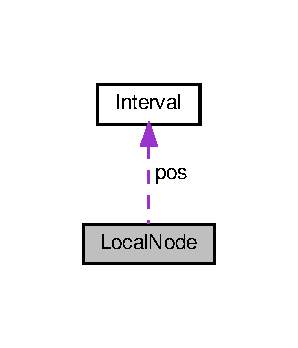
\includegraphics[width=143pt]{classLocalNode__coll__graph}
\end{center}
\end{figure}
\subsection*{Public Member Functions}
\begin{DoxyCompactItemize}
\item 
\mbox{\Hypertarget{classLocalNode_a2802a95378b038d09ba861467621d9d6}\label{classLocalNode_a2802a95378b038d09ba861467621d9d6}} 
{\bfseries Local\+Node} (std\+::string, \hyperlink{structInterval}{Interval}, uint32\+\_\+t)
\item 
\mbox{\Hypertarget{classLocalNode_a363824a550915c6a5874489571a6efe3}\label{classLocalNode_a363824a550915c6a5874489571a6efe3}} 
bool {\bfseries operator==} (const \hyperlink{classLocalNode}{Local\+Node} \&y) const
\end{DoxyCompactItemize}
\subsection*{Public Attributes}
\begin{DoxyCompactItemize}
\item 
\mbox{\Hypertarget{classLocalNode_ab9782768a6be08070824665ef747239f}\label{classLocalNode_ab9782768a6be08070824665ef747239f}} 
std\+::string {\bfseries seq}
\item 
\mbox{\Hypertarget{classLocalNode_af2831e1ceeaea3a483e8777f4e78d178}\label{classLocalNode_af2831e1ceeaea3a483e8777f4e78d178}} 
\hyperlink{structInterval}{Interval} {\bfseries pos}
\item 
\mbox{\Hypertarget{classLocalNode_a6d01c5dabe54dfd97ff0592c5c193463}\label{classLocalNode_a6d01c5dabe54dfd97ff0592c5c193463}} 
uint32\+\_\+t {\bfseries id}
\item 
\mbox{\Hypertarget{classLocalNode_a9e10522ae9782ec417b91837f0f874c8}\label{classLocalNode_a9e10522ae9782ec417b91837f0f874c8}} 
uint32\+\_\+t {\bfseries covg}
\item 
\mbox{\Hypertarget{classLocalNode_aa8bd262ead3022ae143543d53dd9183c}\label{classLocalNode_aa8bd262ead3022ae143543d53dd9183c}} 
uint32\+\_\+t {\bfseries sketch\+\_\+next}
\item 
\mbox{\Hypertarget{classLocalNode_ac99a8a8eae84ee90cf4b0aa45d049a5f}\label{classLocalNode_ac99a8a8eae84ee90cf4b0aa45d049a5f}} 
bool {\bfseries skip}
\item 
\mbox{\Hypertarget{classLocalNode_afa38aeb939508833afdca842f42f9dad}\label{classLocalNode_afa38aeb939508833afdca842f42f9dad}} 
std\+::vector$<$ Local\+Node\+Ptr $>$ {\bfseries out\+Nodes}
\end{DoxyCompactItemize}
\subsection*{Friends}
\begin{DoxyCompactItemize}
\item 
\mbox{\Hypertarget{classLocalNode_aac1fc722ed62c9cdcec0a666cbee3277}\label{classLocalNode_aac1fc722ed62c9cdcec0a666cbee3277}} 
class {\bfseries Local\+Graph}
\item 
\mbox{\Hypertarget{classLocalNode_a99a72d107e31f7e3824a18ff7af2fbc5}\label{classLocalNode_a99a72d107e31f7e3824a18ff7af2fbc5}} 
class {\bfseries Local\+P\+RG}
\item 
\mbox{\Hypertarget{classLocalNode_a5e360852aa8d9c98f1be6b16d4c03d21}\label{classLocalNode_a5e360852aa8d9c98f1be6b16d4c03d21}} 
std\+::ostream \& {\bfseries operator$<$$<$} (std\+::ostream \&out, const \hyperlink{classLocalNode}{Local\+Node} \&n)
\end{DoxyCompactItemize}


The documentation for this class was generated from the following files\+:\begin{DoxyCompactItemize}
\item 
include/localnode.\+h\item 
src/localnode.\+cpp\end{DoxyCompactItemize}

\hypertarget{classLocalPRG}{}\section{Local\+P\+RG Class Reference}
\label{classLocalPRG}\index{Local\+P\+RG@{Local\+P\+RG}}


Collaboration diagram for Local\+P\+RG\+:\nopagebreak
\begin{figure}[H]
\begin{center}
\leavevmode
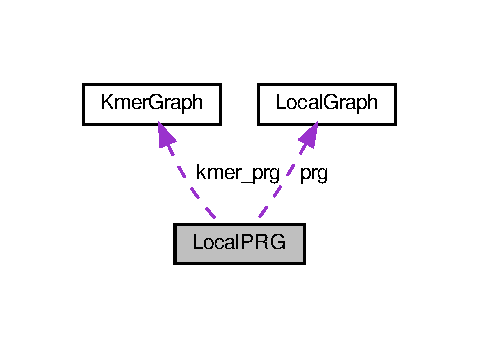
\includegraphics[width=230pt]{classLocalPRG__coll__graph}
\end{center}
\end{figure}
\subsection*{Public Member Functions}
\begin{DoxyCompactItemize}
\item 
\mbox{\Hypertarget{classLocalPRG_a1729caff2615403d128a1eef7315e628}\label{classLocalPRG_a1729caff2615403d128a1eef7315e628}} 
{\bfseries Local\+P\+RG} (uint32\+\_\+t, const std\+::string \&, const std\+::string \&)
\item 
\mbox{\Hypertarget{classLocalPRG_a66967eea834a60152a06d7fa86e6acf4}\label{classLocalPRG_a66967eea834a60152a06d7fa86e6acf4}} 
bool {\bfseries isalpha\+\_\+string} (const std\+::string \&) const
\item 
\mbox{\Hypertarget{classLocalPRG_a8041fa9e8e7778df63717ae6f42e2a2d}\label{classLocalPRG_a8041fa9e8e7778df63717ae6f42e2a2d}} 
std\+::string {\bfseries string\+\_\+along\+\_\+path} (const prg\+::\+Path \&) const
\item 
\mbox{\Hypertarget{classLocalPRG_ad32899108525a9513bccfd28dc88bb55}\label{classLocalPRG_ad32899108525a9513bccfd28dc88bb55}} 
std\+::vector$<$ Local\+Node\+Ptr $>$ {\bfseries nodes\+\_\+along\+\_\+path} (const prg\+::\+Path \&) const
\item 
\mbox{\Hypertarget{classLocalPRG_a8754af497c7dfa032180aab230409915}\label{classLocalPRG_a8754af497c7dfa032180aab230409915}} 
std\+::vector$<$ \hyperlink{structInterval}{Interval} $>$ {\bfseries split\+\_\+by\+\_\+site} (const \hyperlink{structInterval}{Interval} \&) const
\item 
\mbox{\Hypertarget{classLocalPRG_a3b66546b0da44781f6b5c0dd1c25642d}\label{classLocalPRG_a3b66546b0da44781f6b5c0dd1c25642d}} 
std\+::vector$<$ uint32\+\_\+t $>$ {\bfseries build\+\_\+graph} (const \hyperlink{structInterval}{Interval} \&, const std\+::vector$<$ uint32\+\_\+t $>$ \&, uint32\+\_\+t current\+\_\+level=0)
\item 
\mbox{\Hypertarget{classLocalPRG_a3474c581e00373d41ec304ee3886b1c6}\label{classLocalPRG_a3474c581e00373d41ec304ee3886b1c6}} 
std\+::vector$<$ prg\+::\+Path $>$ {\bfseries shift} (prg\+::\+Path) const
\item 
\mbox{\Hypertarget{classLocalPRG_a9873a8f72a0bea283e6f399078b08f60}\label{classLocalPRG_a9873a8f72a0bea283e6f399078b08f60}} 
void {\bfseries minimizer\+\_\+sketch} (std\+::shared\+\_\+ptr$<$ \hyperlink{classIndex}{Index} $>$ index, const uint32\+\_\+t w, const uint32\+\_\+t k)
\item 
\mbox{\Hypertarget{classLocalPRG_a73008cf730eb3c8f4ebb15850a056430}\label{classLocalPRG_a73008cf730eb3c8f4ebb15850a056430}} 
std\+::vector$<$ Kmer\+Node\+Ptr $>$ {\bfseries kmernode\+\_\+path\+\_\+from\+\_\+localnode\+\_\+path} (const std\+::vector$<$ Local\+Node\+Ptr $>$ \&) const
\item 
\mbox{\Hypertarget{classLocalPRG_a28119980b89df2c53712298451289f00}\label{classLocalPRG_a28119980b89df2c53712298451289f00}} 
std\+::vector$<$ Local\+Node\+Ptr $>$ {\bfseries localnode\+\_\+path\+\_\+from\+\_\+kmernode\+\_\+path} (const std\+::vector$<$ Kmer\+Node\+Ptr $>$ \&, const uint32\+\_\+t w=0) const
\item 
\mbox{\Hypertarget{classLocalPRG_a1869125941195fc0546e972281931839}\label{classLocalPRG_a1869125941195fc0546e972281931839}} 
void {\bfseries write\+\_\+covgs\+\_\+to\+\_\+file} (const boost\+::filesystem\+::path \&, const std\+::vector$<$ uint32\+\_\+t $>$ \&) const
\item 
\mbox{\Hypertarget{classLocalPRG_a02cfae8a258d05fb0f0883702a61d027}\label{classLocalPRG_a02cfae8a258d05fb0f0883702a61d027}} 
void {\bfseries write\+\_\+path\+\_\+to\+\_\+fasta} (const boost\+::filesystem\+::path \&, const std\+::vector$<$ Local\+Node\+Ptr $>$ \&, const float \&) const
\item 
\mbox{\Hypertarget{classLocalPRG_ad53a06335e970239bae28ea38a06193f}\label{classLocalPRG_ad53a06335e970239bae28ea38a06193f}} 
void {\bfseries append\+\_\+path\+\_\+to\+\_\+fasta} (const boost\+::filesystem\+::path \&, const std\+::vector$<$ Local\+Node\+Ptr $>$ \&, const float \&) const
\item 
\mbox{\Hypertarget{classLocalPRG_aae75df1603fddd25ff06f4fdab369fec}\label{classLocalPRG_aae75df1603fddd25ff06f4fdab369fec}} 
void {\bfseries write\+\_\+aligned\+\_\+path\+\_\+to\+\_\+fasta} (const boost\+::filesystem\+::path \&, const std\+::vector$<$ Local\+Node\+Ptr $>$ \&, const float \&) const
\item 
\mbox{\Hypertarget{classLocalPRG_ac4f8dfb2555af538ac2b89a7b414788f}\label{classLocalPRG_ac4f8dfb2555af538ac2b89a7b414788f}} 
void {\bfseries build\+\_\+vcf} (\hyperlink{classVCF}{V\+CF} \&, const std\+::vector$<$ Local\+Node\+Ptr $>$ \&) const
\item 
\mbox{\Hypertarget{classLocalPRG_a989f2128badfd99b3600d99b21dfa9e6}\label{classLocalPRG_a989f2128badfd99b3600d99b21dfa9e6}} 
void {\bfseries add\+\_\+sample\+\_\+gt\+\_\+to\+\_\+vcf} (\hyperlink{classVCF}{V\+CF} \&, const std\+::vector$<$ Local\+Node\+Ptr $>$ \&, const std\+::vector$<$ Local\+Node\+Ptr $>$ \&, const std\+::string \&sample\+\_\+name=\char`\"{}sample\char`\"{}) const
\item 
\mbox{\Hypertarget{classLocalPRG_a5f3dbbd8e8c5d7571847957ff401e83b}\label{classLocalPRG_a5f3dbbd8e8c5d7571847957ff401e83b}} 
std\+::vector$<$ Local\+Node\+Ptr $>$ {\bfseries find\+\_\+alt\+\_\+path} (const std\+::vector$<$ Local\+Node\+Ptr $>$ \&, const uint32\+\_\+t, const std\+::string \&, const std\+::string \&) const
\item 
\mbox{\Hypertarget{classLocalPRG_ad9f3b252cdbb7d23fb36543917c0bc0a}\label{classLocalPRG_ad9f3b252cdbb7d23fb36543917c0bc0a}} 
void {\bfseries append\+\_\+kmer\+\_\+covgs\+\_\+in\+\_\+range} (const \hyperlink{classKmerGraph}{Kmer\+Graph} \&, const std\+::vector$<$ Kmer\+Node\+Ptr $>$ \&, const std\+::vector$<$ Local\+Node\+Ptr $>$ \&, const uint32\+\_\+t \&, const uint32\+\_\+t \&, std\+::vector$<$ uint32\+\_\+t $>$ \&, std\+::vector$<$ uint32\+\_\+t $>$ \&) const
\item 
\mbox{\Hypertarget{classLocalPRG_ab38532465665803109701ca3166b67c8}\label{classLocalPRG_ab38532465665803109701ca3166b67c8}} 
void {\bfseries add\+\_\+sample\+\_\+covgs\+\_\+to\+\_\+vcf} (\hyperlink{classVCF}{V\+CF} \&, const \hyperlink{classKmerGraph}{Kmer\+Graph} \&, const std\+::vector$<$ Local\+Node\+Ptr $>$ \&, const std\+::string \&sample\+\_\+name=\char`\"{}sample\char`\"{}) const
\item 
\mbox{\Hypertarget{classLocalPRG_a6cf906c1307763026cf185f07d8eace7}\label{classLocalPRG_a6cf906c1307763026cf185f07d8eace7}} 
void {\bfseries add\+\_\+consensus\+\_\+path\+\_\+to\+\_\+fastaq} (\hyperlink{structFastaq}{Fastaq} \&, Pan\+Node\+Ptr, std\+::vector$<$ Kmer\+Node\+Ptr $>$ \&, std\+::vector$<$ Local\+Node\+Ptr $>$ \&, const uint32\+\_\+t w, const bool bin=false, const uint32\+\_\+t global\+\_\+covg=1)
\item 
\mbox{\Hypertarget{classLocalPRG_a0f1b2f176fc2c36bd05f7caca3c8127e}\label{classLocalPRG_a0f1b2f176fc2c36bd05f7caca3c8127e}} 
void {\bfseries add\+\_\+variants\+\_\+to\+\_\+vcf} (\hyperlink{classVCF}{V\+CF} \&, Pan\+Node\+Ptr, const std\+::string \&, const std\+::vector$<$ Kmer\+Node\+Ptr $>$ \&, const std\+::vector$<$ Local\+Node\+Ptr $>$ \&, const std\+::string \&sample\+\_\+name=\char`\"{}sample\char`\"{})
\end{DoxyCompactItemize}
\subsection*{Static Public Member Functions}
\begin{DoxyCompactItemize}
\item 
\mbox{\Hypertarget{classLocalPRG_a44590a1c176f93c150cc8137a98f52c7}\label{classLocalPRG_a44590a1c176f93c150cc8137a98f52c7}} 
static std\+::string {\bfseries string\+\_\+along\+\_\+path} (const std\+::vector$<$ Local\+Node\+Ptr $>$ \&)
\end{DoxyCompactItemize}
\subsection*{Public Attributes}
\begin{DoxyCompactItemize}
\item 
\mbox{\Hypertarget{classLocalPRG_abf9e601dc3d00bb4e574da95324cbc15}\label{classLocalPRG_abf9e601dc3d00bb4e574da95324cbc15}} 
uint32\+\_\+t {\bfseries next\+\_\+site}
\item 
\mbox{\Hypertarget{classLocalPRG_ae0b0928141665bf209eba94cb46972a2}\label{classLocalPRG_ae0b0928141665bf209eba94cb46972a2}} 
uint32\+\_\+t {\bfseries id}
\item 
\mbox{\Hypertarget{classLocalPRG_a101b866a36a0721ad6985c0442f9ac10}\label{classLocalPRG_a101b866a36a0721ad6985c0442f9ac10}} 
std\+::string {\bfseries name}
\item 
\mbox{\Hypertarget{classLocalPRG_a1a32007bf210ecb5b06e135aca50a372}\label{classLocalPRG_a1a32007bf210ecb5b06e135aca50a372}} 
std\+::string {\bfseries seq}
\item 
\mbox{\Hypertarget{classLocalPRG_a0c3ca6e8a8568a7bb2d8f5860d29aa45}\label{classLocalPRG_a0c3ca6e8a8568a7bb2d8f5860d29aa45}} 
\hyperlink{classLocalGraph}{Local\+Graph} {\bfseries prg}
\item 
\mbox{\Hypertarget{classLocalPRG_aef3aece10be2745d990a37913011f5a9}\label{classLocalPRG_aef3aece10be2745d990a37913011f5a9}} 
\hyperlink{classKmerGraph}{Kmer\+Graph} {\bfseries kmer\+\_\+prg}
\item 
\mbox{\Hypertarget{classLocalPRG_a276b54851100a10b334306856bfb230d}\label{classLocalPRG_a276b54851100a10b334306856bfb230d}} 
std\+::vector$<$ uint32\+\_\+t $>$ {\bfseries num\+\_\+hits}
\end{DoxyCompactItemize}
\subsection*{Friends}
\begin{DoxyCompactItemize}
\item 
\mbox{\Hypertarget{classLocalPRG_a8f0ba3182680e495c26f00482617b684}\label{classLocalPRG_a8f0ba3182680e495c26f00482617b684}} 
std\+::ostream \& {\bfseries operator$<$$<$} (std\+::ostream \&out, const \hyperlink{classLocalPRG}{Local\+P\+RG} \&data)
\end{DoxyCompactItemize}


The documentation for this class was generated from the following files\+:\begin{DoxyCompactItemize}
\item 
include/local\+P\+R\+G.\+h\item 
src/local\+P\+R\+G.\+cpp\end{DoxyCompactItemize}

\hypertarget{structMinimizer}{}\section{Minimizer Struct Reference}
\label{structMinimizer}\index{Minimizer@{Minimizer}}


Collaboration diagram for Minimizer\+:\nopagebreak
\begin{figure}[H]
\begin{center}
\leavevmode
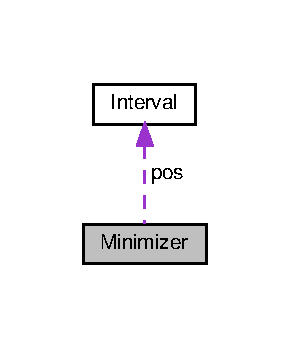
\includegraphics[width=139pt]{structMinimizer__coll__graph}
\end{center}
\end{figure}
\subsection*{Public Member Functions}
\begin{DoxyCompactItemize}
\item 
\mbox{\Hypertarget{structMinimizer_a9af8fbb16263bf9b0f1ca04db4e1aead}\label{structMinimizer_a9af8fbb16263bf9b0f1ca04db4e1aead}} 
{\bfseries Minimizer} (uint64\+\_\+t, uint32\+\_\+t, uint32\+\_\+t, bool)
\item 
\mbox{\Hypertarget{structMinimizer_a59a496028328f1dc79f76a4b9417bfde}\label{structMinimizer_a59a496028328f1dc79f76a4b9417bfde}} 
bool {\bfseries operator$<$} (const \hyperlink{structMinimizer}{Minimizer} \&y) const
\item 
\mbox{\Hypertarget{structMinimizer_a4a7c2e2df1f20e6a8ed8fb08be44c4f1}\label{structMinimizer_a4a7c2e2df1f20e6a8ed8fb08be44c4f1}} 
bool {\bfseries operator==} (const \hyperlink{structMinimizer}{Minimizer} \&y) const
\end{DoxyCompactItemize}
\subsection*{Public Attributes}
\begin{DoxyCompactItemize}
\item 
\mbox{\Hypertarget{structMinimizer_a5a1897a6ab2a57f299cacd201b5488ac}\label{structMinimizer_a5a1897a6ab2a57f299cacd201b5488ac}} 
uint64\+\_\+t {\bfseries kmer}
\item 
\mbox{\Hypertarget{structMinimizer_a4096a676386cd7176bda788b2651986b}\label{structMinimizer_a4096a676386cd7176bda788b2651986b}} 
\hyperlink{structInterval}{Interval} {\bfseries pos}
\item 
\mbox{\Hypertarget{structMinimizer_a1f98393ca75068179f896cb96073d659}\label{structMinimizer_a1f98393ca75068179f896cb96073d659}} 
bool {\bfseries strand}
\end{DoxyCompactItemize}
\subsection*{Friends}
\begin{DoxyCompactItemize}
\item 
\mbox{\Hypertarget{structMinimizer_abaa955320c5133352a39fbb9e372638b}\label{structMinimizer_abaa955320c5133352a39fbb9e372638b}} 
std\+::ostream \& {\bfseries operator$<$$<$} (std\+::ostream \&out, const \hyperlink{structMinimizer}{Minimizer} \&m)
\end{DoxyCompactItemize}


The documentation for this struct was generated from the following files\+:\begin{DoxyCompactItemize}
\item 
include/minimizer.\+h\item 
src/minimizer.\+cpp\end{DoxyCompactItemize}

\hypertarget{structMinimizerHit}{}\section{Minimizer\+Hit Struct Reference}
\label{structMinimizerHit}\index{Minimizer\+Hit@{Minimizer\+Hit}}
\subsection*{Public Member Functions}
\begin{DoxyCompactItemize}
\item 
\mbox{\Hypertarget{structMinimizerHit_a33d7f08088357743c067a95ca37625a9}\label{structMinimizerHit_a33d7f08088357743c067a95ca37625a9}} 
{\bfseries Minimizer\+Hit} (const uint32\+\_\+t i, const \hyperlink{structMinimizer}{Minimizer} \&m, const \hyperlink{structMiniRecord}{Mini\+Record} $\ast$r)
\item 
\mbox{\Hypertarget{structMinimizerHit_acdb79c266210dfaaa2dce35f2097b9fc}\label{structMinimizerHit_acdb79c266210dfaaa2dce35f2097b9fc}} 
{\bfseries Minimizer\+Hit} (const uint32\+\_\+t i, const \hyperlink{structInterval}{Interval} j, const uint32\+\_\+t k, const prg\+::\+Path p, const uint32\+\_\+t n, const bool c)
\item 
\mbox{\Hypertarget{structMinimizerHit_af1a85716a5696e7ca0d9cc27ef321446}\label{structMinimizerHit_af1a85716a5696e7ca0d9cc27ef321446}} 
bool {\bfseries operator$<$} (const \hyperlink{structMinimizerHit}{Minimizer\+Hit} \&y) const
\item 
\mbox{\Hypertarget{structMinimizerHit_ac06296d203dc8cdde9dcd4733be524b5}\label{structMinimizerHit_ac06296d203dc8cdde9dcd4733be524b5}} 
bool {\bfseries operator==} (const \hyperlink{structMinimizerHit}{Minimizer\+Hit} \&y) const
\end{DoxyCompactItemize}
\subsection*{Public Attributes}
\begin{DoxyCompactItemize}
\item 
\mbox{\Hypertarget{structMinimizerHit_a4be91f378dd1ecf3fa6524fc66a06834}\label{structMinimizerHit_a4be91f378dd1ecf3fa6524fc66a06834}} 
uint32\+\_\+t {\bfseries read\+\_\+id}
\item 
\mbox{\Hypertarget{structMinimizerHit_ac71537bc57caef0dc26da9d02c1dfc7d}\label{structMinimizerHit_ac71537bc57caef0dc26da9d02c1dfc7d}} 
uint32\+\_\+t {\bfseries read\+\_\+start\+\_\+position}
\item 
\mbox{\Hypertarget{structMinimizerHit_aafb1dc2d20eaa1c590c5cd53fa1193dc}\label{structMinimizerHit_aafb1dc2d20eaa1c590c5cd53fa1193dc}} 
uint32\+\_\+t {\bfseries prg\+\_\+id}
\item 
\mbox{\Hypertarget{structMinimizerHit_a7bb0a2cc7a47c4dded7e807b5b69e4bf}\label{structMinimizerHit_a7bb0a2cc7a47c4dded7e807b5b69e4bf}} 
prg\+::\+Path {\bfseries prg\+\_\+path}
\item 
\mbox{\Hypertarget{structMinimizerHit_aa1682626b80f6376844d97f1a9c19816}\label{structMinimizerHit_aa1682626b80f6376844d97f1a9c19816}} 
uint32\+\_\+t {\bfseries knode\+\_\+id}
\item 
\mbox{\Hypertarget{structMinimizerHit_a0743c359476e41278b084dbe8a24b9c1}\label{structMinimizerHit_a0743c359476e41278b084dbe8a24b9c1}} 
bool {\bfseries strand}
\end{DoxyCompactItemize}
\subsection*{Friends}
\begin{DoxyCompactItemize}
\item 
\mbox{\Hypertarget{structMinimizerHit_ad6546ef24569abacf9851ff95f68c498}\label{structMinimizerHit_ad6546ef24569abacf9851ff95f68c498}} 
std\+::ostream \& {\bfseries operator$<$$<$} (std\+::ostream \&out, const \hyperlink{structMinimizerHit}{Minimizer\+Hit} \&m)
\end{DoxyCompactItemize}


The documentation for this struct was generated from the following files\+:\begin{DoxyCompactItemize}
\item 
include/minihit.\+h\item 
src/minihit.\+cpp\end{DoxyCompactItemize}

\hypertarget{classMinimizerHits}{}\section{Minimizer\+Hits Class Reference}
\label{classMinimizerHits}\index{Minimizer\+Hits@{Minimizer\+Hits}}
\subsection*{Public Member Functions}
\begin{DoxyCompactItemize}
\item 
\mbox{\Hypertarget{classMinimizerHits_a7eb7b8fc345f22900966dd3063f672f0}\label{classMinimizerHits_a7eb7b8fc345f22900966dd3063f672f0}} 
{\bfseries Minimizer\+Hits} (const uint32\+\_\+t \&num\+\_\+hits=30000)
\item 
\mbox{\Hypertarget{classMinimizerHits_ac37a6dea43f610d2c2f938979128b7ad}\label{classMinimizerHits_ac37a6dea43f610d2c2f938979128b7ad}} 
void {\bfseries clear} ()
\item 
\mbox{\Hypertarget{classMinimizerHits_a086b03a37004125711335a4f1f4bb250}\label{classMinimizerHits_a086b03a37004125711335a4f1f4bb250}} 
void {\bfseries add\+\_\+hit} (const uint32\+\_\+t i, const \hyperlink{structMinimizer}{Minimizer} \&m, const \hyperlink{structMiniRecord}{Mini\+Record} $\ast$r)
\item 
\mbox{\Hypertarget{classMinimizerHits_a258cf9fca5922ced1d278e88650502db}\label{classMinimizerHits_a258cf9fca5922ced1d278e88650502db}} 
void {\bfseries sort} ()
\end{DoxyCompactItemize}
\subsection*{Public Attributes}
\begin{DoxyCompactItemize}
\item 
\mbox{\Hypertarget{classMinimizerHits_a496389f6989e628b660448644bc1728a}\label{classMinimizerHits_a496389f6989e628b660448644bc1728a}} 
std\+::unordered\+\_\+set$<$ Minimizer\+Hit\+Ptr $>$ {\bfseries uhits}
\item 
\mbox{\Hypertarget{classMinimizerHits_aa3724c783e03e19c37851e458f36f205}\label{classMinimizerHits_aa3724c783e03e19c37851e458f36f205}} 
std\+::set$<$ Minimizer\+Hit\+Ptr, \hyperlink{structpComp}{p\+Comp} $>$ {\bfseries hits}
\end{DoxyCompactItemize}
\subsection*{Friends}
\begin{DoxyCompactItemize}
\item 
\mbox{\Hypertarget{classMinimizerHits_a909db7b6fd1771335ed163db5d65d583}\label{classMinimizerHits_a909db7b6fd1771335ed163db5d65d583}} 
std\+::ostream \& {\bfseries operator$<$$<$} (std\+::ostream \&out, const \hyperlink{classMinimizerHits}{Minimizer\+Hits} \&m)
\end{DoxyCompactItemize}


The documentation for this class was generated from the following files\+:\begin{DoxyCompactItemize}
\item 
include/minihits.\+h\item 
src/minihits.\+cpp\end{DoxyCompactItemize}

\hypertarget{structMiniRecord}{}\section{Mini\+Record Struct Reference}
\label{structMiniRecord}\index{Mini\+Record@{Mini\+Record}}
\subsection*{Public Member Functions}
\begin{DoxyCompactItemize}
\item 
\mbox{\Hypertarget{structMiniRecord_a768a1f3044350283ca5f25d7032985ed}\label{structMiniRecord_a768a1f3044350283ca5f25d7032985ed}} 
{\bfseries Mini\+Record} (const uint32\+\_\+t, const Path, const uint32\+\_\+t, const bool)
\item 
\mbox{\Hypertarget{structMiniRecord_ab7056477df9b306a890ee80096485b47}\label{structMiniRecord_ab7056477df9b306a890ee80096485b47}} 
bool {\bfseries operator==} (const \hyperlink{structMiniRecord}{Mini\+Record} \&y) const
\end{DoxyCompactItemize}
\subsection*{Public Attributes}
\begin{DoxyCompactItemize}
\item 
\mbox{\Hypertarget{structMiniRecord_aef0452bf5833638a93af53bdac3c898c}\label{structMiniRecord_aef0452bf5833638a93af53bdac3c898c}} 
uint32\+\_\+t {\bfseries prg\+\_\+id}
\item 
\mbox{\Hypertarget{structMiniRecord_aa890b6bfa4a505214aa50f9f70f91b5d}\label{structMiniRecord_aa890b6bfa4a505214aa50f9f70f91b5d}} 
Path {\bfseries path}
\item 
\mbox{\Hypertarget{structMiniRecord_a97e2c87da5af20abad25c2c08036bb3a}\label{structMiniRecord_a97e2c87da5af20abad25c2c08036bb3a}} 
uint32\+\_\+t {\bfseries knode\+\_\+id}
\item 
\mbox{\Hypertarget{structMiniRecord_a76c6269939e525768647df5751afd019}\label{structMiniRecord_a76c6269939e525768647df5751afd019}} 
bool {\bfseries strand}
\end{DoxyCompactItemize}
\subsection*{Friends}
\begin{DoxyCompactItemize}
\item 
\mbox{\Hypertarget{structMiniRecord_adf1a022fece5080694a3eddd02925038}\label{structMiniRecord_adf1a022fece5080694a3eddd02925038}} 
std\+::ostream \& {\bfseries operator$<$$<$} (std\+::ostream \&out, const \hyperlink{structMiniRecord}{Mini\+Record} \&m)
\item 
\mbox{\Hypertarget{structMiniRecord_a5d9e09fdb821d377589ebb60a846089b}\label{structMiniRecord_a5d9e09fdb821d377589ebb60a846089b}} 
std\+::istream \& {\bfseries operator$>$$>$} (std\+::istream \&in, \hyperlink{structMiniRecord}{Mini\+Record} \&m)
\end{DoxyCompactItemize}


The documentation for this struct was generated from the following files\+:\begin{DoxyCompactItemize}
\item 
include/minirecord.\+h\item 
src/minirecord.\+cpp\end{DoxyCompactItemize}

\hypertarget{structpComp}{}\section{p\+Comp Struct Reference}
\label{structpComp}\index{p\+Comp@{p\+Comp}}
\subsection*{Public Member Functions}
\begin{DoxyCompactItemize}
\item 
\mbox{\Hypertarget{structpComp_ae587ce6fb6b5bf3595f9c00934628f8e}\label{structpComp_ae587ce6fb6b5bf3595f9c00934628f8e}} 
bool {\bfseries operator()} (const Minimizer\+Hit\+Ptr \&lhs, const Minimizer\+Hit\+Ptr \&rhs)
\end{DoxyCompactItemize}


The documentation for this struct was generated from the following files\+:\begin{DoxyCompactItemize}
\item 
include/minihits.\+h\item 
src/minihits.\+cpp\end{DoxyCompactItemize}

\hypertarget{structpComp__path}{}\section{p\+Comp\+\_\+path Struct Reference}
\label{structpComp__path}\index{p\+Comp\+\_\+path@{p\+Comp\+\_\+path}}
\subsection*{Public Member Functions}
\begin{DoxyCompactItemize}
\item 
\mbox{\Hypertarget{structpComp__path_a60987a68b6b2fed0e213da00499fe212}\label{structpComp__path_a60987a68b6b2fed0e213da00499fe212}} 
bool {\bfseries operator()} (const Minimizer\+Hit\+Ptr \&lhs, const Minimizer\+Hit\+Ptr \&rhs)
\end{DoxyCompactItemize}


The documentation for this struct was generated from the following files\+:\begin{DoxyCompactItemize}
\item 
include/minihits.\+h\item 
src/minihits.\+cpp\end{DoxyCompactItemize}

\hypertarget{structpCompKmerNode}{}\section{p\+Comp\+Kmer\+Node Struct Reference}
\label{structpCompKmerNode}\index{p\+Comp\+Kmer\+Node@{p\+Comp\+Kmer\+Node}}
\subsection*{Public Member Functions}
\begin{DoxyCompactItemize}
\item 
\mbox{\Hypertarget{structpCompKmerNode_a31eb79aeb16c8dddc59a2dee12d74a3f}\label{structpCompKmerNode_a31eb79aeb16c8dddc59a2dee12d74a3f}} 
bool {\bfseries operator()} (Kmer\+Node\+Ptr, Kmer\+Node\+Ptr)
\end{DoxyCompactItemize}


The documentation for this struct was generated from the following files\+:\begin{DoxyCompactItemize}
\item 
include/kmergraph.\+h\item 
src/kmergraph.\+cpp\end{DoxyCompactItemize}

\hypertarget{structpEq}{}\section{p\+Eq Struct Reference}
\label{structpEq}\index{p\+Eq@{p\+Eq}}
\subsection*{Public Member Functions}
\begin{DoxyCompactItemize}
\item 
\mbox{\Hypertarget{structpEq_a3414473a7c7825f9d71d02a5dbb899c7}\label{structpEq_a3414473a7c7825f9d71d02a5dbb899c7}} 
bool {\bfseries operator()} (const Minimizer\+Hit\+Ptr \&lhs, const Minimizer\+Hit\+Ptr \&rhs) const
\end{DoxyCompactItemize}


The documentation for this struct was generated from the following files\+:\begin{DoxyCompactItemize}
\item 
include/minihits.\+h\item 
src/minihits.\+cpp\end{DoxyCompactItemize}

\hypertarget{structpointer__values__equal}{}\section{pointer\+\_\+values\+\_\+equal$<$ T $>$ Struct Template Reference}
\label{structpointer__values__equal}\index{pointer\+\_\+values\+\_\+equal$<$ T $>$@{pointer\+\_\+values\+\_\+equal$<$ T $>$}}
\subsection*{Public Member Functions}
\begin{DoxyCompactItemize}
\item 
\mbox{\Hypertarget{structpointer__values__equal_af5907ba14fa25c5714e6b032122b9c1b}\label{structpointer__values__equal_af5907ba14fa25c5714e6b032122b9c1b}} 
bool {\bfseries operator()} (const T $\ast$other) const
\end{DoxyCompactItemize}
\subsection*{Public Attributes}
\begin{DoxyCompactItemize}
\item 
\mbox{\Hypertarget{structpointer__values__equal_a08b86fa4873efed09a79b79786164f29}\label{structpointer__values__equal_a08b86fa4873efed09a79b79786164f29}} 
const T $\ast$ {\bfseries to\+\_\+find}
\end{DoxyCompactItemize}


The documentation for this struct was generated from the following file\+:\begin{DoxyCompactItemize}
\item 
include/utils.\+h\end{DoxyCompactItemize}

\hypertarget{classSeq}{}\section{Seq Class Reference}
\label{classSeq}\index{Seq@{Seq}}
\subsection*{Public Member Functions}
\begin{DoxyCompactItemize}
\item 
\mbox{\Hypertarget{classSeq_a3a0b4b1578f2dd9fd369bad28a2f81df}\label{classSeq_a3a0b4b1578f2dd9fd369bad28a2f81df}} 
{\bfseries Seq} (uint32\+\_\+t, std\+::string, std\+::string, uint32\+\_\+t, uint32\+\_\+t)
\item 
\mbox{\Hypertarget{classSeq_a6cc4fcb51f6c8df1c01b577c7b4dab13}\label{classSeq_a6cc4fcb51f6c8df1c01b577c7b4dab13}} 
void {\bfseries initialize} (uint32\+\_\+t, std\+::string, std\+::string, uint32\+\_\+t, uint32\+\_\+t)
\item 
\mbox{\Hypertarget{classSeq_a63222414c30166df6a600d1026f7b9be}\label{classSeq_a63222414c30166df6a600d1026f7b9be}} 
bool {\bfseries add\+\_\+letter\+\_\+to\+\_\+get\+\_\+next\+\_\+kmer} (const char \&, const uint64\+\_\+t \&, const uint64\+\_\+t \&, uint32\+\_\+t \&, uint64\+\_\+t(\&)\mbox{[}2\mbox{]}, uint64\+\_\+t(\&)\mbox{[}2\mbox{]})
\item 
\mbox{\Hypertarget{classSeq_abd7c9d3b5d760d8faabbb00fa52b2a56}\label{classSeq_abd7c9d3b5d760d8faabbb00fa52b2a56}} 
void {\bfseries add\+\_\+minimizing\+\_\+kmers\+\_\+to\+\_\+sketch} (const std\+::vector$<$ \hyperlink{structMinimizer}{Minimizer} $>$ \&, const uint64\+\_\+t \&)
\item 
\mbox{\Hypertarget{classSeq_a35c3c8d99777c39df5343603b87a7e54}\label{classSeq_a35c3c8d99777c39df5343603b87a7e54}} 
void {\bfseries minimize\+\_\+window} (std\+::vector$<$ \hyperlink{structMinimizer}{Minimizer} $>$ \&, uint64\+\_\+t \&)
\item 
\mbox{\Hypertarget{classSeq_a3c90f2abd6ab7bcd1dcb788a3423a388}\label{classSeq_a3c90f2abd6ab7bcd1dcb788a3423a388}} 
void {\bfseries add\+\_\+new\+\_\+smallest\+\_\+minimizer} (std\+::vector$<$ \hyperlink{structMinimizer}{Minimizer} $>$ \&, uint64\+\_\+t \&)
\item 
\mbox{\Hypertarget{classSeq_a00227ec5e397a525f727be95aa4c6b3e}\label{classSeq_a00227ec5e397a525f727be95aa4c6b3e}} 
void {\bfseries minimizer\+\_\+sketch} (const uint32\+\_\+t w, const uint32\+\_\+t k)
\end{DoxyCompactItemize}
\subsection*{Public Attributes}
\begin{DoxyCompactItemize}
\item 
\mbox{\Hypertarget{classSeq_a92ca613f18683745cfdc9c0e41b19c75}\label{classSeq_a92ca613f18683745cfdc9c0e41b19c75}} 
uint32\+\_\+t {\bfseries id}
\item 
\mbox{\Hypertarget{classSeq_ac609fcce0f7b2460dccb093b2c5c11b8}\label{classSeq_ac609fcce0f7b2460dccb093b2c5c11b8}} 
std\+::string {\bfseries name}
\item 
\mbox{\Hypertarget{classSeq_af6aa27e38a75f7294882d86883246d00}\label{classSeq_af6aa27e38a75f7294882d86883246d00}} 
std\+::string {\bfseries seq}
\item 
\mbox{\Hypertarget{classSeq_a0ec0bde4a1631fd67eeede750f8a8c05}\label{classSeq_a0ec0bde4a1631fd67eeede750f8a8c05}} 
std\+::set$<$ \hyperlink{structMinimizer}{Minimizer} $>$ {\bfseries sketch}
\end{DoxyCompactItemize}
\subsection*{Friends}
\begin{DoxyCompactItemize}
\item 
\mbox{\Hypertarget{classSeq_a09c523f7cdc8313b2b2ac1dac4cbf1d4}\label{classSeq_a09c523f7cdc8313b2b2ac1dac4cbf1d4}} 
std\+::ostream \& {\bfseries operator$<$$<$} (std\+::ostream \&out, const \hyperlink{classSeq}{Seq} \&data)
\end{DoxyCompactItemize}


The documentation for this class was generated from the following files\+:\begin{DoxyCompactItemize}
\item 
include/seq.\+h\item 
src/seq.\+cpp\end{DoxyCompactItemize}

\hypertarget{structspointer__values__equal}{}\section{spointer\+\_\+values\+\_\+equal$<$ T $>$ Struct Template Reference}
\label{structspointer__values__equal}\index{spointer\+\_\+values\+\_\+equal$<$ T $>$@{spointer\+\_\+values\+\_\+equal$<$ T $>$}}
\subsection*{Public Member Functions}
\begin{DoxyCompactItemize}
\item 
\mbox{\Hypertarget{structspointer__values__equal_a60d5052ca3584627868cb4114dd8fb4b}\label{structspointer__values__equal_a60d5052ca3584627868cb4114dd8fb4b}} 
bool {\bfseries operator()} (const std\+::shared\+\_\+ptr$<$ T $>$ other) const
\end{DoxyCompactItemize}
\subsection*{Public Attributes}
\begin{DoxyCompactItemize}
\item 
\mbox{\Hypertarget{structspointer__values__equal_acbf739f5bf9651671603b3cc6b467136}\label{structspointer__values__equal_acbf739f5bf9651671603b3cc6b467136}} 
const std\+::shared\+\_\+ptr$<$ T $>$ {\bfseries to\+\_\+find}
\end{DoxyCompactItemize}


The documentation for this struct was generated from the following file\+:\begin{DoxyCompactItemize}
\item 
include/utils.\+h\end{DoxyCompactItemize}

\hypertarget{classVCF}{}\section{V\+CF Class Reference}
\label{classVCF}\index{V\+CF@{V\+CF}}
\subsection*{Public Member Functions}
\begin{DoxyCompactItemize}
\item 
\mbox{\Hypertarget{classVCF_a84fc6c1a477d10f747d0facb0096d194}\label{classVCF_a84fc6c1a477d10f747d0facb0096d194}} 
void {\bfseries add\+\_\+record} (std\+::string c, uint32\+\_\+t p, std\+::string r, std\+::string a, std\+::string i=\char`\"{}.\char`\"{}, std\+::string g=\char`\"{}\char`\"{})
\item 
\mbox{\Hypertarget{classVCF_a57edaedcef6bfffb4ee1ae9f82b2f282}\label{classVCF_a57edaedcef6bfffb4ee1ae9f82b2f282}} 
\hyperlink{structVCFRecord}{V\+C\+F\+Record} \& {\bfseries add\+\_\+record} (\hyperlink{structVCFRecord}{V\+C\+F\+Record} \&)
\item 
\mbox{\Hypertarget{classVCF_a150ea8b5fd1312540d2845746ed21159}\label{classVCF_a150ea8b5fd1312540d2845746ed21159}} 
void {\bfseries add\+\_\+formats} (const std\+::vector$<$ std\+::string $>$ \&)
\item 
\mbox{\Hypertarget{classVCF_a0890d71a1603151c9092db244864bf5f}\label{classVCF_a0890d71a1603151c9092db244864bf5f}} 
ptrdiff\+\_\+t {\bfseries get\+\_\+sample\+\_\+index} (const std\+::string \&)
\item 
\mbox{\Hypertarget{classVCF_aaabe5597d48f4cca5da9f259d252eb5a}\label{classVCF_aaabe5597d48f4cca5da9f259d252eb5a}} 
void {\bfseries add\+\_\+sample\+\_\+gt} (const std\+::string \&name, const std\+::string \&c, const uint32\+\_\+t p, const std\+::string \&r, const std\+::string \&a)
\item 
\mbox{\Hypertarget{classVCF_ab17bda29f53e402d65e07e7f30cbc7d6}\label{classVCF_ab17bda29f53e402d65e07e7f30cbc7d6}} 
void {\bfseries add\+\_\+sample\+\_\+ref\+\_\+alleles} (const std\+::string \&, const std\+::string \&, const uint32\+\_\+t \&, const uint32\+\_\+t \&)
\item 
\mbox{\Hypertarget{classVCF_acc69ff06098d92e28bfc7433aca9370d}\label{classVCF_acc69ff06098d92e28bfc7433aca9370d}} 
void {\bfseries clear} ()
\item 
\mbox{\Hypertarget{classVCF_a508cf00e71166cad0e00350082f32982}\label{classVCF_a508cf00e71166cad0e00350082f32982}} 
void {\bfseries append\+\_\+vcf} (const \hyperlink{classVCF}{V\+CF} \&)
\item 
\mbox{\Hypertarget{classVCF_a1d357c818e4a6de958350985ca85f19a}\label{classVCF_a1d357c818e4a6de958350985ca85f19a}} 
void {\bfseries sort\+\_\+records} ()
\item 
\mbox{\Hypertarget{classVCF_a533bba4aca3713e4459b2175071a5539}\label{classVCF_a533bba4aca3713e4459b2175071a5539}} 
bool {\bfseries pos\+\_\+in\+\_\+range} (const uint32\+\_\+t, const uint32\+\_\+t, const std\+::string \&) const
\item 
\mbox{\Hypertarget{classVCF_a225a043c79990aba1f13a299eb346445}\label{classVCF_a225a043c79990aba1f13a299eb346445}} 
void {\bfseries genotype} (const uint32\+\_\+t \&, const float \&, const uint8\+\_\+t, bool snps\+\_\+only=true)
\item 
\mbox{\Hypertarget{classVCF_a908fce1dfb9d0eef4f956430dda8b232}\label{classVCF_a908fce1dfb9d0eef4f956430dda8b232}} 
void {\bfseries clean} ()
\item 
\mbox{\Hypertarget{classVCF_ab83cca445adf503d609d0a30d6456358}\label{classVCF_ab83cca445adf503d609d0a30d6456358}} 
void {\bfseries merge\+\_\+multi\+\_\+allelic} (uint32\+\_\+t max\+\_\+allele\+\_\+length=10000)
\item 
\mbox{\Hypertarget{classVCF_ac0a8bd5b103f7837616b1c7a8269950c}\label{classVCF_ac0a8bd5b103f7837616b1c7a8269950c}} 
void {\bfseries make\+\_\+gt\+\_\+compatible} ()
\item 
\mbox{\Hypertarget{classVCF_a14a2d3805017bceee9eff41e39bf98a5}\label{classVCF_a14a2d3805017bceee9eff41e39bf98a5}} 
std\+::string {\bfseries header} ()
\item 
\mbox{\Hypertarget{classVCF_a2ccca210cdfd1f8a667abaa569161cb5}\label{classVCF_a2ccca210cdfd1f8a667abaa569161cb5}} 
void {\bfseries save} (const std\+::string \&, bool simple=false, bool complexgraph=false, bool toomanyalts=false, bool snp=false, bool indel=false, bool phsnps=false, bool complexvar=false)
\item 
\mbox{\Hypertarget{classVCF_a9fd1ea9c320328019fababacc7ccc2ca}\label{classVCF_a9fd1ea9c320328019fababacc7ccc2ca}} 
void {\bfseries load} (const std\+::string \&)
\item 
\mbox{\Hypertarget{classVCF_a32b580e2e2e22abddce35d916a865eb6}\label{classVCF_a32b580e2e2e22abddce35d916a865eb6}} 
bool {\bfseries operator==} (const \hyperlink{classVCF}{V\+CF} \&y) const
\item 
\mbox{\Hypertarget{classVCF_a7abcb6100aeb61c9a305b11df90880e7}\label{classVCF_a7abcb6100aeb61c9a305b11df90880e7}} 
bool {\bfseries operator!=} (const \hyperlink{classVCF}{V\+CF} \&y) const
\end{DoxyCompactItemize}
\subsection*{Public Attributes}
\begin{DoxyCompactItemize}
\item 
\mbox{\Hypertarget{classVCF_ab8f80911b0f85d25cf5db5c9ae3a9fde}\label{classVCF_ab8f80911b0f85d25cf5db5c9ae3a9fde}} 
std\+::vector$<$ \hyperlink{structVCFRecord}{V\+C\+F\+Record} $>$ {\bfseries records}
\item 
\mbox{\Hypertarget{classVCF_a919f0d1cd538ec4a52fc4c45a7db0148}\label{classVCF_a919f0d1cd538ec4a52fc4c45a7db0148}} 
std\+::vector$<$ std\+::string $>$ {\bfseries samples}
\end{DoxyCompactItemize}
\subsection*{Friends}
\begin{DoxyCompactItemize}
\item 
\mbox{\Hypertarget{classVCF_a5aee2ddd11bc238dc603ec57bebf9cbb}\label{classVCF_a5aee2ddd11bc238dc603ec57bebf9cbb}} 
std\+::ostream \& {\bfseries operator$<$$<$} (std\+::ostream \&out, const \hyperlink{classVCF}{V\+CF} \&m)
\end{DoxyCompactItemize}


The documentation for this class was generated from the following files\+:\begin{DoxyCompactItemize}
\item 
include/vcf.\+h\item 
src/vcf.\+cpp\end{DoxyCompactItemize}

\hypertarget{structVCFRecord}{}\section{V\+C\+F\+Record Struct Reference}
\label{structVCFRecord}\index{V\+C\+F\+Record@{V\+C\+F\+Record}}
\subsection*{Public Member Functions}
\begin{DoxyCompactItemize}
\item 
\mbox{\Hypertarget{structVCFRecord_ae5fb81c0b593d1e21b046e336b5ce51a}\label{structVCFRecord_ae5fb81c0b593d1e21b046e336b5ce51a}} 
{\bfseries V\+C\+F\+Record} (std\+::string, uint32\+\_\+t, std\+::string, std\+::string, std\+::string i=\char`\"{}.\char`\"{}, std\+::string g=\char`\"{}\char`\"{})
\item 
\mbox{\Hypertarget{structVCFRecord_af3f3230f9ecc1c99c5e543fb72e6f787}\label{structVCFRecord_af3f3230f9ecc1c99c5e543fb72e6f787}} 
{\bfseries V\+C\+F\+Record} (const \hyperlink{structVCFRecord}{V\+C\+F\+Record} \&)
\item 
\mbox{\Hypertarget{structVCFRecord_a84cd091176e34ef977ed1b54f2710c83}\label{structVCFRecord_a84cd091176e34ef977ed1b54f2710c83}} 
\hyperlink{structVCFRecord}{V\+C\+F\+Record} \& {\bfseries operator=} (const \hyperlink{structVCFRecord}{V\+C\+F\+Record} \&)
\item 
\mbox{\Hypertarget{structVCFRecord_a30453a7d38b7b95de34ae5d0c829ceca}\label{structVCFRecord_a30453a7d38b7b95de34ae5d0c829ceca}} 
void {\bfseries clear} ()
\item 
\mbox{\Hypertarget{structVCFRecord_a320f11b04c13945685257623b1998bec}\label{structVCFRecord_a320f11b04c13945685257623b1998bec}} 
void {\bfseries clear\+\_\+sample} (uint32\+\_\+t)
\item 
\mbox{\Hypertarget{structVCFRecord_af4975a1462b648fac35ec293f74f4709}\label{structVCFRecord_af4975a1462b648fac35ec293f74f4709}} 
void {\bfseries add\+\_\+formats} (const std\+::vector$<$ std\+::string $>$ \&)
\item 
\mbox{\Hypertarget{structVCFRecord_aa8d663da339a028347efa387fcd0180c}\label{structVCFRecord_aa8d663da339a028347efa387fcd0180c}} 
void {\bfseries likelihood} (const uint32\+\_\+t \&, const float \&)
\item 
\mbox{\Hypertarget{structVCFRecord_aae4066c90ccaa1512826159efebc1524}\label{structVCFRecord_aae4066c90ccaa1512826159efebc1524}} 
void {\bfseries confidence} ()
\item 
\mbox{\Hypertarget{structVCFRecord_a87f07cb0e91691bc4b97d962a2938f81}\label{structVCFRecord_a87f07cb0e91691bc4b97d962a2938f81}} 
void {\bfseries genotype} (const uint8\+\_\+t)
\item 
\mbox{\Hypertarget{structVCFRecord_a2118c8363d1879b7fba3ebe999664bb6}\label{structVCFRecord_a2118c8363d1879b7fba3ebe999664bb6}} 
bool {\bfseries operator==} (const \hyperlink{structVCFRecord}{V\+C\+F\+Record} \&y) const
\item 
\mbox{\Hypertarget{structVCFRecord_acd81c197de30dce551e663fd69d79263}\label{structVCFRecord_acd81c197de30dce551e663fd69d79263}} 
bool {\bfseries operator!=} (const \hyperlink{structVCFRecord}{V\+C\+F\+Record} \&y) const
\item 
\mbox{\Hypertarget{structVCFRecord_a8368290aa1815ef6ea71881691a17440}\label{structVCFRecord_a8368290aa1815ef6ea71881691a17440}} 
bool {\bfseries operator$<$} (const \hyperlink{structVCFRecord}{V\+C\+F\+Record} \&y) const
\end{DoxyCompactItemize}
\subsection*{Public Attributes}
\begin{DoxyCompactItemize}
\item 
\mbox{\Hypertarget{structVCFRecord_a87e885f47dc0da6dc4fdb4075c9d466e}\label{structVCFRecord_a87e885f47dc0da6dc4fdb4075c9d466e}} 
std\+::string {\bfseries chrom}
\item 
\mbox{\Hypertarget{structVCFRecord_a41ac8eac6775ce7afe405f046912a5b0}\label{structVCFRecord_a41ac8eac6775ce7afe405f046912a5b0}} 
uint32\+\_\+t {\bfseries pos}
\item 
\mbox{\Hypertarget{structVCFRecord_a56e46ffd2d833a84b599878b01812289}\label{structVCFRecord_a56e46ffd2d833a84b599878b01812289}} 
std\+::string {\bfseries id}
\item 
\mbox{\Hypertarget{structVCFRecord_ab4136d5f6754eb70022230fba89eb4f2}\label{structVCFRecord_ab4136d5f6754eb70022230fba89eb4f2}} 
std\+::string {\bfseries ref}
\item 
\mbox{\Hypertarget{structVCFRecord_a3d608f0c7886d1dd1610a8e9b09e22c6}\label{structVCFRecord_a3d608f0c7886d1dd1610a8e9b09e22c6}} 
std\+::vector$<$ std\+::string $>$ {\bfseries alt}
\item 
\mbox{\Hypertarget{structVCFRecord_a687c908f41401cc70a1021fbc4544ebd}\label{structVCFRecord_a687c908f41401cc70a1021fbc4544ebd}} 
std\+::string {\bfseries qual}
\item 
\mbox{\Hypertarget{structVCFRecord_af85743e9a6e36f61a3ca3e6b97aca54a}\label{structVCFRecord_af85743e9a6e36f61a3ca3e6b97aca54a}} 
std\+::string {\bfseries filter}
\item 
\mbox{\Hypertarget{structVCFRecord_a48a47329fc5a33844260cb0b10785d1c}\label{structVCFRecord_a48a47329fc5a33844260cb0b10785d1c}} 
std\+::string {\bfseries info}
\item 
\mbox{\Hypertarget{structVCFRecord_a751a843dc16b746713fe03539ec901bb}\label{structVCFRecord_a751a843dc16b746713fe03539ec901bb}} 
std\+::vector$<$ std\+::string $>$ {\bfseries format}
\item 
\mbox{\Hypertarget{structVCFRecord_a4dc33f496f4bfd9882ae21ce9ad5b428}\label{structVCFRecord_a4dc33f496f4bfd9882ae21ce9ad5b428}} 
std\+::vector$<$ std\+::unordered\+\_\+map$<$ std\+::string, std\+::vector$<$ uint8\+\_\+t $>$ $>$ $>$ {\bfseries samples}
\item 
\mbox{\Hypertarget{structVCFRecord_a382c0585ecc43021ca65c023076c8070}\label{structVCFRecord_a382c0585ecc43021ca65c023076c8070}} 
std\+::vector$<$ std\+::unordered\+\_\+map$<$ std\+::string, std\+::vector$<$ float $>$ $>$ $>$ {\bfseries regt\+\_\+samples}
\end{DoxyCompactItemize}
\subsection*{Friends}
\begin{DoxyCompactItemize}
\item 
\mbox{\Hypertarget{structVCFRecord_adebe668cf2281b4b9c10e50032adedba}\label{structVCFRecord_adebe668cf2281b4b9c10e50032adedba}} 
std\+::ostream \& {\bfseries operator$<$$<$} (std\+::ostream \&out, const \hyperlink{structVCFRecord}{V\+C\+F\+Record} \&m)
\item 
\mbox{\Hypertarget{structVCFRecord_a446bcf6252d8ff2d3e2e0823114ff821}\label{structVCFRecord_a446bcf6252d8ff2d3e2e0823114ff821}} 
std\+::istream \& {\bfseries operator$>$$>$} (std\+::istream \&in, \hyperlink{structVCFRecord}{V\+C\+F\+Record} \&m)
\end{DoxyCompactItemize}


The documentation for this struct was generated from the following files\+:\begin{DoxyCompactItemize}
\item 
include/vcfrecord.\+h\item 
src/vcfrecord.\+cpp\end{DoxyCompactItemize}

%--- End generated contents ---

% Index
\backmatter
\newpage
\phantomsection
\clearemptydoublepage
\addcontentsline{toc}{chapter}{Index}
\printindex

\end{document}
